% vim: ft=tex expandtab

\documentclass[12pt]{report}
\usepackage[utf8]{inputenc}
\usepackage[serbian]{babel}
\usepackage[backend=biber, style=numeric, sorting=none]{biblatex}
\usepackage{csquotes}
\usepackage[a4paper, top=20mm, bottom=20mm, left=30mm, right=15mm, headheight=10mm, headsep=5mm, footskip=9mm]{geometry}
\usepackage{fancyhdr}
\usepackage{float}
\usepackage{fontspec}
\usepackage[acronym]{glossaries}
\usepackage{graphicx}
\usepackage{hyperref}
\usepackage{titlesec}
\usepackage{ragged2e}
\usepackage{setspace}

\hypersetup{hidelinks}

\setmainfont{Times New Roman}

\tolerance=1
\emergencystretch=\maxdimen
\hyphenpenalty=10000
\hbadness=10000

\addbibresource{literature.bib}

\pagestyle{fancy}

\renewcommand{\chaptermark}[1]{\markboth{#1}{}}
\renewcommand{\sectionmark}[1]{\markright{\arabic{section}.\ #1}}
\renewcommand{\baselinestretch}{1.4}
\newcommand{\normal}{
\tolerance=1
\emergencystretch=\maxdimen
}

\makeatletter
\newcommand\frontmatter{
    \cleardoublepage{}
    \pagenumbering{Roman}
    \setlength{\parskip}{0pt}
}

\setsansfont{Arial}

\newcommand\mainmatter{
    \cleardoublepage{}
    \pagenumbering{arabic}
    \setlength{\parskip}{2mm}
    \titleformat{\chapter}{\normalfont\Large\bf\sffamily\raggedleft}{\thechapter.}{12pt}{}
}
\makeatother

\titlespacing*{\chapter}{0mm}{58mm}{10mm}
\titleformat{\chapter}{\normalfont\Large\bf\sffamily}{\thechapter.}{12pt}{}
\titleformat{\section}{\normalfont\large\bf\sffamily}{\thesection}{12pt}{}
\titleformat{\subsection}{\normalfont\bf\sffamily}{\thesubsection}{12pt}{}
\titleformat{\subsubsection}{\normalfont\bf\sffamily}{\thesubsubsection}{12pt}{}
\setcounter{secnumdepth}{4}

\fancypagestyle{plain}{}
\fancyhead[L]{}
\fancyhead[R]{\leftmark}
\fancyfoot{}
\fancyfoot[R]{\thepage}

\raggedbottom{}

\begin{document}

\frontmatter{}

\renewcommand{\MakeUppercase}[1]{#1}
\tableofcontents

\listoffigures

\chapter*{Skraćenice}
\chaptermark{Skraćenice}
\begin{tabular}{ l l }
    \textbf{API} & -- \textit{Application programming interface}, Interfejs za programiranje aplikacija \\
    \textbf{CLI} & -- \textit{Command line interface}, Interfejs komandne linije \\
    \textbf{GCC} & -- \textit{GNU compiler collection}, GNU kolekcija kompajlera \\
    \textbf{PDF} & -- \textit{Portable Document Format}, Portabilni format dokumenata \\
    \textbf{URL} & -- \textit{Uniform resource locator}, Jedinstveni lokator resursa \\
    \textbf{YAML} & -- \textit{YAML Ain't Markup Languag}, YAML nije jezik za označavanje \\
\end{tabular}

\mainmatter{}
\chapter{Uvod}
Od samog početka razvoja računarstva, ideja je bila da računari i softverski alati koji se na njima koriste olakšaju ljudske aktivnosti koje zahtevaju mnogo uloženog vremena ili resursa da bi se izvršile jednom ili više puta. Ove aktivnosti su vremenom postajale sve kompleksnije, a alati koji ih rešavaju sve moćniji. Jedan od takvih alata, koji je nastao pre svega nekoliko meseci, su GitHub akcije.

Zadatak ovog rada je da kroz realan primer razvoja softvera otvorenog koda (eng.\ \textit{open-source}) testira primer upotrebe Github akcija i sve prednosti i mane koje ovaj alat donosi. Projekat otvorenog koda koji se koristi u ovom primeru je \textit{pjisp-assignment-template}. U pitanju je softverski alat koji se koristi za automatizovano kreiranja zadataka za studente korišćenjem šablona na predmetu Programski jezici i strukture podataka na Fakultetu tehničkih nauka u Novom Sadu.

Proces kreiranja zadatka upotrebom \textit{pjisp-assignment-template} alata sastoji se iz nekoliko koraka, te postoji mogućnost da se napravi greška. Pomoću GitHub akcija, u malopre pomenuti alat se integrišu drugi alati, koji služe za vršenje provera ispravnosti nekih od koraka i koji dodatno olakšavaju proces kreiranja zadatka. Ovi alati predstavljaju programe koji se mogu instalirati i nezavisno od \textit{pjisp-assignment-template} alata, a i sami za pripremanje izvršne verzije koriste GitHub akcije.

Ovaj rad opisuje sve prethodno pomenute alate, tehnologije koje se koriste za njihovu implementaciju i način njihove integracije u celinu upotrebom GitHub akcija. Na kraju samog rada, izvedeni su zaključci o GitHub akcijama stečeni na osnovu njihovog korišćenja u procesu izrade ovog rada.

\chapter{Teorijske osnove}
U ovom poglavlju će biti ukratko objašnjeni svi koncepti i alati koji su bili potrebni za izradu projekta o kojem ovaj rad govori. Tu grupu čini pre svega Softver otvorenog koda kao koncept pod kojim je ovaj projekat razvijen. Zatim se navode osnove karakteristike Sistema za praćenje verzija datoteka i Git kao glavni predstavnik takvih sistema. Naredno poglavlje se nadovezuje pričom o GitHub-u. Sledećih nekoliko poglavlja se bave Python programskim jezikom, njegovim paketima, repozitorijumom za te pakete i alatima za upravljanje paketima - Poetry-jem i Pipenv-om. Poslednje poglavlje opisuje Bash jezik komandne linije.

\section{Softver otvorenog koda}
Pojam otvoreni kod se odnosi na nešto što je dostupno svima za pravljenje izmena ili deljenje. Javio se kao pojam vezan za razvoj softvera (eng.\ \textit{software}), ali se danas koristi i u drugim kontekstima vezanim za otvorenost i dostupnost.

Softver otvorenog koda je sotver čiji izvorni kod svako može da posmatra, menja, poboljšava, ispravlja greske, dodaje nove funkcionalnosti, itd. Ovakav softver se objavljuje pod licencama otvorenog koda. Ove licence dozvoljavaju korišćenje i deljenje koda pod određenim uslovima. Najčešće se kodu može pristupiti besplatno. Nekada se licencom zahteva da se kod koristi samo u nekomercijalne svrhe ili da se navede originalni autor koda. Često licenca traži i da se izmenjeni kod deli pod istom tom licencom.

Pogodnosti pisanja i korišćenja ovakvog koda su mnogobrojne, a ovo su neke od njih:

\begin{itemize}
    \item \textbf{Kontrola} - Korisnici softvera otvorenog koda imaju uvid u kod koji koriste, i samim tim veću kontrolu nad onim što instaliraju i koriste na svojim računarima. Takođe, mogu da menjaju delove koda koji im se ne dopadaju.
    \item \textbf{Učenje} - Dostupnost koda omogućava korisnicima da analiziraju kod i time postaju bolji programeri. Takođe, pisanjem softvera otvorenog koda, korisnici ostavljaju mogućnost drugim korisnicima da vide njihov kod i da im daju sugestije/kritike. Pri pronalaženju grešaka u kodu, korisnici mogu da ih podele sa drugima i time spreče druge korisnike u pravljenju istih grešaka.
    \item \textbf{Bezbednost} - Mnogi smatraju softver otvorenog koda bezbednijim od softvera zatvorenog koda. Zato što je kod javan i dostupan svima za izmene, postoji mogućnost da će neko od korisnika pronaći i ispraviti propuste koje autor nije primetio. Takođe, nađene greške se brže ispravljaju pošto nema potrebe da se čeka na autora koda da ih ispravi, već to može da uradi bilo ko.
    \item \textbf{Stabilnost} - Softver otvorenog koda se takođe smatra stabilnijim i pouzdanijim rešenjem za projekte koji treba da se koriste dugi niz godina. Čak i ako originalni autor koda odustane od razvoja, postoji velika mogućnost da će neko od korisnika i učesnika nastaviti da ga održava.
    \item \textbf{Zajednica} - Oko softvera otvorenog koda često se formira zajednica korisnika i učesnika u razvoju koda. To su ljudi koji pišu, testiraju i koriste kod i zajedno razmenjuju ideje o poboljšanjima projekta i napretku.
\end{itemize}

\section{Sistem za praćenje verzija datoteka}
Sistem za praćenje verzija datoteka (eng.\ \textit{version control system}) je sistem zadužen za praćenje istorije promena u datotekama. Promena koja se pamti se najčešće naziva revizija. Sve promene se uglavnom čuvaju na centralizovanom sistemu za skladištenje podataka i svi korisnici sa potrebnim privilegijama mogu da mu pristupaju, preuzmu sve nove revizije i primene ih na lokalnim datotekama, izmene lokalne datoteke i zatim objave novu reviziju koja se od tog momenta smatra najnovijom.

U ovim sistemima, čuva se celokupna istorija promena i moguće je vratiti datoteke u bilo koju od prethodnih revizija. U pogledu softvera, ovo nam omogućava da vratimo u upotrebu bilo koju prethodnu verziju, u slučaju da dođe do greške u nekoj od novijih verzija. Istorija se čuva u strukturi tipa grafa:

\begin{figure}[H]
    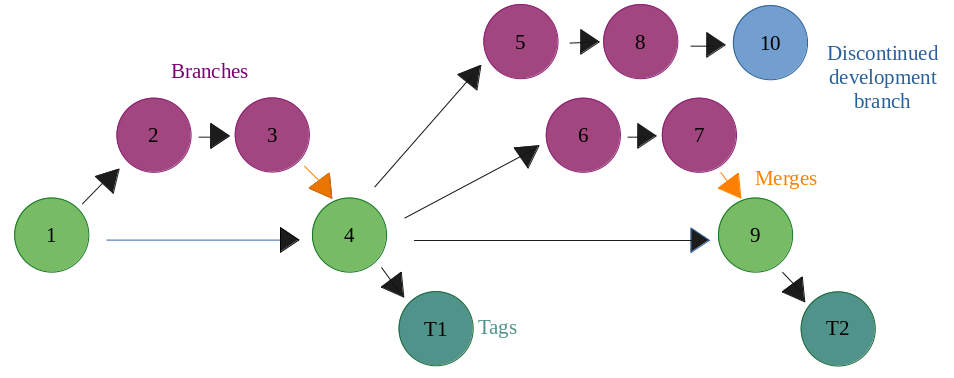
\includegraphics[width=\linewidth]{images/version_control.png}
    \caption{Sistem za praćenje verzija datoteka}
\end{figure}

Graf se najčešće sastoji od glavne grane (eng.\ \textit{branch}), na kojoj se nalaze glavne izmene, i pomoćnih grana na kojima se nalaze izmene za koje još nije odlučeno da li će pripadati glavnoj grani. Ako sve izmene na pomoćnim granama budu odgovarajuće, one se spajaju (eng.\ \textit{merge}) sa glavnom granom i postaju deo njenog sadržaja. U slučaju praćenja verzija softvera, ovakve grane najčešće predstavljaju nove funkcionalnosti (eng.\ \textit{feature}) koje se dodaju na glavnu granu projekta ili ispravljanje greške (eng.\ \textit{bugfix}) koja je nastala u nekoj od prethodnih verzija.

Važne izmene se mogu dodatno naglasiti dodavanjem priveska (eng.\ \textit{tag}). One uglavnom predstavljaju objavljivanje nove verzije softvera (eng.\ \textit{release}), dodavanje nove funkcionalnosti ili ispravku greške.

\section{Git}
Git \cite{git} je besplatan softver otvorenog koda za praćenje verzija datoteka u distribuiranom režimu. Primarno se koristi za razvoj softvera, ali se može koristiti i za praćenje bilo kojih drugih datoteka. Razvoj je započeo 2005. godine kreator Linux-a, Linus Torvalds, za potrebe razvoja jezgra Linux operativnog sistema. Distribuiran je pod GNU General Public License Version 2 licencom. Primarno je napravljen za Linux operativni sistem, ali je naknadno prilagođen i za macOS, BSD, Solaris i Windows.

Za razliku od drugih sistema za praćenje verzija datoteka u distribuiranom režimu, Git nije softver klijent-server arhitekture. Svaki Git repozitorijum na svakom računaru čuva kompletnu istoriju promena i verzija i nije zavisan od pristupa mreži ili centralizovanom serveru. Kao takav, Git je osnova za razvoj mnogih drugih nezavisnih alata za praćenje verzija datoteka.

\section{GitHub}
GitHub \cite{github} je servis otvorenog koda za hostovanje (eng.\ \textit{hosting}) repozitorijuma sa različitim datotekama, najčešće izvornim kodovima za razna softverska rešenja. Za praćenje verzija datoteka, GitHub koristi Git. GitHub služi kao centralizovano mesto na kojem se čuvaju i razmenjuju sve izmene koje su sačuvane upotrebom Git alata.

U ovom trenutku, GitHub se smatra najpopularnijim alatom ovog tipa i trenutno broji preko 40 miliona korisnika. Stvari koje ovaj servis omogućava su:

\begin{enumerate}
    \item Upravljanje projektima
    \item Upravljanje timom
    \item Pregled i komentarisanje koda
    \item Integracija
    \item Paketi
    \item Bezbednost
    \item Hostovanje
    \item Akcije
\end{enumerate}

Moguće mu je pristupiti preko CLI verzije, desktop verzije, ekstenzije za Visual Studio program za uređivanje datoteka (eng.\ \textit{text editor}) i mobilne aplikacije.

\subsection{Upravljanje projektima}
Upravljanje projektom je proces koji je potreban u bilo kojem većem programerskom projektu. Menadžeri projekta su zaduženi da prate razvoj projekta i upućuju programere u razvoj narednih delova projekata, kao i da upravljaju raspoređivanjem vremena rada na različitim zadacima koje projekat iziskuje.

GitHub nudi mogućnost koordinacije projektom, praćenje razvoja i menjanje statusa projekta na jednom mestu. Koordinacija započinje kreiranjem zadataka (eng.\ \textit{tasks}) koji traže izmene koda ili unapređenja projekta. Zadaci mogu biti u obliku greške/pitanja (eng.\ \textit{issue}), komentara (eng.\ \textit{comment}) ili zahteva za izmenom (eng.\ \textit{pull-request}), što podrazumeva kreiranje celine koja je spremna za spajanje sa glavnom granom na projektu. Zadacima se dodeljuju osobe koje su zadužene za njih. Time će oni dobijati obaveštenja kada dođe do bilo koje izmene u projektu vezane za njihov deo posla. Zadacima je moguće dodeliti i prioritet i oznake (eng.\ \textit{label}), što dodatno olakšava proces upravljanja projektom.

Sve ove informacije moguće je pratiti i menjati u formi tabele (eng.\ \textit{board}) ili u repozitorijumu na kojem se projekat nalazi. Svaki zadatak ima unikatan URL na kojem se mogu videti sve potrebne informacije vezane za njega. Čuva se i istorija svih zadataka i izmena na projektu, kojima se stvara uvid u proces razvoja projekta. Po završetku svih zadataka, upravljanje projektom se završava i projekat se označava kao završen.

\subsection{Upravljanje timom}
Kako u timu imamo različite uloge, koje imaju različite permisije, GitHub nudi mogućnost hijerarhijskog organizovanja učesnika na projektu gde se svakoj grupi učesnika ili pojedincu dodeljuju potrebna prava.

Takođe, moguće je dodati u repozitorijum dokumente koji se tiču projekta, kao što su kodeks ponašanja (eng.\ \textit{code of conduct}) i licenca (eng.\ \textit{license}). Ove dokumente nije potrebno svaki put pisati iznova, već postoje unapred predefinisane verzije često korišćenih kodeksa ponašanja i licenci.

\subsection{Pregled i komentarisanje koda}
Komunikacija između učesnika na projektu doprinosi kvalitetu izrade samog projekta. Pored podele zadataka i raspoređivanja vremena za svaki zadatak, javlja se potreba i za diskutovanjem koda koji se dodaje u obliku zahteva za izmenom.

Pri kreiranju zahteva za izmenom ili revizija (eng.\ \textit{commit}), GitHub nudi prikaz svih izmena u odnosu na granu sa koje su izmene krenule i na koju bi se dodale ako je sve u redu. Taj prikaz je dostupan svima koji učestvuju u izradi projekta. Moguće je, dodatno, zamoliti nekoga od učesnika da pregleda izmene pre njihovog spajanja sa odabranom granom (eng.\ \textit{request a review}). Na svakoj od izmena, moguće je dodati poruku, koja otvara mogućnost diskusije sa ostalim učesnicima projekta. Po završetku, osoba koja je zadužena da pregleda izmene može da odobri ili odbije zahtev za izmenom, uz mogućnost traženja dodatnih izmena pre odobrenja.

Takođe, pri kreiranju zahteva za izmenom, GitHub automatski pregleda kod u potrazi za bezbednosnim propustima ili konfliktima sa granom sa kojom se trenutna grana spaja. Ako ih ima, GitHub obaveštava korisnika i traži izmenu pre odobrenja i spajanja koda.

\subsection{Integracija}
Pored samog pisanja aplikacije, često se javlja potreba za testiranjem i praćenjem (eng.\ \textit{monitoring}) aplikacije, automatizovanim postavljanjem u produkciju (eng.\ \textit{deployment}), kontinualnom integracijom (eng.\ \textit{continuous integration}), proverom kvaliteta koda (eng.\ \textit{code quality}) i drugim pomoćnim aktivnostima u procesu razvoja softver-a.

Pošto GitHub nije u mogućnosti da ponudi sve te aktivnosti, omogućio je proces integracije sa servisima koji ih nude. Svi ovi servisi mogu se pronaći u GitHub prodavnici (eng.\ \textit{marketplace}) \cite{marketplace}. Jedna od novina u GitHub prodavnici su GitHub akcije koje će biti jedna od centralnih tema ovog rada, a biće opisane u jednoj od narednih sekcija.

\subsection{Paketi}
Alati poput NPM-a, Docker-a, Maven-a, Gradle-a i drugih omogućavaju kreiranje artifakta koji sadrže sve potrebne alate za pokretanje nekog softverskog rešenja. Većina ovakvih servisa ima mogućnost čuvanja artifakta na njihovim repozitorijumima.

Zbog jednostavnosti korišćenja, GitHub je kreirao alat koji objedinjuje mnoge ovakve repozitorijume u jedan repozitorijum - GitHub Packages.

\subsection{Bezbednost}
Bezbednost u softverskim rešenjima igra veoma bitnu ulogu i najčešće zavisi od mnogo faktora: programera, ljudi koji održavaju kod (eng.\ \textit{maintainers}), istraživača, timova specijalizovanih za bezbednost i drugih. Da bi se postigao što veći stepen bezbednosti, potrebno je da što više različitih strana učestvuje u testiranju koda na bezbednosne propuste (eng.\ \textit{vulnerabilities}).

Neke od mogućnosti koje GitHub nudi za poboljšanje bezbednosti koda koji se nalazi na njemu su:

\begin{itemize}
    \item \textbf{Automatsko skeniranje koda} - pri dodavanju koda na repozitorijum, pokreće se automatsko skeniranje koda na poznate bezbednosne propuste i obaveštava se korisnik ako se pronađe neki od njih
    \item \textbf{Definisanje bezbednosnog procesa rada projekata otvorenog koda} - omogućava definisanje bezbednosnih polisa u okviru \textit{SECURITY.MD} datoteke u repozitorijumu u kojoj se navode sve potrebne informacije o tome koje bezbednosne probleme i na koji način treba da prijave korisnici koji ih pronađu
    \item \textbf{Diskutovanje o uticaju bezbednosnih propusta} - kada neki od korisnika prijavi bezbednosni propust ili grešku u kodu, GitHub nudi prostor za komentarisanje i razmenu mišljenja vezanog za postavljeni problem
    \item \textbf{Automatsko skeniranje zavisnosti} - slično skeniranju koda, pokreće se automatsko skeniranje zavisnosti nekog projekta - odnosno svih drugih softverskih rešenja od kojih projekat zavisi. Ako neko od njih ima bezbednosni propust, korisnik se obaveštava o tome. Ovakvi problemi često budu otklonjeni u narednoj verziji rešenja od kojeg projekat zavisi, pa GitHub često nudi promenu verzije kao rešenje ovakvog problema. Ovaj proces se nastavlja za vreme životnog ciklusa projekta, i ako se u bilo kojem momentu pronađe bezbednosni propust, automatski se kreira zahtev za izmenom sa ispravkom
    \item \textbf{Pretraga kredencijala} - korisnicima se može desiti da slučajno upišu kredencijale za neki od eksternih servisa u kod projekta. Takvi kredencijali imaju specifičan oblik koji GitHub prepoznaje za preko 24 servisa i obaveštava korisnika ako ih pronađe
\end{itemize}

\subsection{Hostovanje sajtova}
Pored hostovanja repozitorijuma, što je glavna uloga GitHub-a, postoji i mogućnost hostovanja sajta pod GitHub domenom. Potrebno je napraviti repozitorijum sa nazivom \textit{username.github.io} i svi dokumenti u okviru njega će biti statički hostovani pod \textit{username.github.io} domenom.

\subsection{Akcije}
Kao što vidimo iz prethodnih sekcija, GitHub nudi mnoge mogućnosti pored njegove osnovne namene - praćenja verzija datoteka. Ipak, ako i te mogućnosti nisu dovoljne, postoji alat - GitHub Actions koji nudi mogućnost pisanja tokova posla (eng.\ \textit{workflow}) i reagovanje na mnoge događaje, tako da korisnik može, u specifičnom formatu, da definiše sve potrebne reakcije na događaje i pokrije slučajeve koje ostali GitHub alati ne pokrivaju. Ove akcije najčešće podrazumevaju automatizaciju, podešavanje i izvršavanje delova softverskih rešenja nakon nekog specifičng događaja.

\subsubsection{Događaji}
Neki od događaja na koje je moguće reagovati su:

\begin{itemize}
    \item \texttt{create} - pokreće se izvršavanje svaki put kada se kreira nova grana ili privezak
    \item \texttt{delete} - pokreće se izvršavanje svaki put kada se obriše grana ili privezak
    \item \texttt{fork} - pokreće se izvršavanje pri račvanju novog projekta iz trenutnog projekta
    \item \texttt{gollum} - pokreće se izvršavanje svaki put kada se kreira ili izmeni Wiki stranica vezana za projekat
    \item \texttt{issues} - pokreće se izvršavanje svaki put kada se desi \textit{issue} događaj. što podrazumeva otvaranje teme sa pitanjem, njenu izmenu, zatvaranje, brisanje, dodavanje priveska, itd.
    \item \texttt{issue\_comment} - pokreće se izvršavanje svaki put kada se doda, izmeni ili obriše komentar na otvorenom pitanju
    \item \texttt{label} - pokreće se izvršavanje svaki put kada se doda, izmeni ili obriše oznaka
    \item \texttt{milestone} - pokreće se izvršavanje svaki put kada se doda, izmeni ili obriše prekretnica u projektu
    \item \texttt{project} - pokreće se izvršavanje svaki put kada se desi \textit{project} događaj, što podrazumeva kreiranje, izmenu, zatvaranje ili brisanje projekta
    \item \texttt{public} - pokreće se izvršavanje svaki put kada privatni repozitorijum postane javni
    \item \texttt{pull\_request} - pokreće se izvršavanje svaki put kada se desi \textit{pull\_request} događaj, što podrazumeva otvaranje zahteva za izmenom ili njegovu izmenu, zatvaranje, brisanje, dodeljivanje, dodavanje priveska, sinhronizaciju, traženje pregledanja, itd.
    \item \texttt{pull\_request\_review} - pokreće se izvršavanje kada se izvrši, izmeni ili obriše pregledanje zahteva za izmenom
    \item \texttt{pull\_request\_review\_comment} - pokreće se izvršavanje kada se kreira, izmeni ili obriše komentar na pregledanju zahteva za izmenom
    \item \texttt{push} - pokreće se izvršavanje svaki put kada se doda novi kod na granu
    \item \texttt{registry\_package} - pokreće se izvršavanje svaki put kada se objavi ili izmeni paket
    \item \texttt{release} - pokreće se izvršavanje svaki put kada se desi release događaj, što podrazumeva kreiranje, objavljivanje, izmenu ili brisanje nove verzije projekta
\end{itemize}

Takođe, moguće je zakazati izvršavanje neke akcije navođenjem tačnog datuma i vremena izvršavanja ili zakazivanjem izvršavanja na primer svake nedelje u određeno vreme. Za opisivanje vremena koristi se softverski alat \textit{Cron}, koji je zadužen za planiranje i zakazivanje poslova na osnovu vremena (eng.\ \textit{time-based job scheduler}) na Unix operativnim sistemima.

Tokovi poslova se opisuju u YAML formatu. Događaji se opisuju u okviru \textit{on} sekcije, uz dodatak \textit{type} i \textit{branch} podsekcija ako ima potrebe. Na primer:

\begin{samepage}
    \begin{verbatim}
    on:
        pull_request:
            branches:
            - master
        release:
            types:
            - created
    \end{verbatim}
\end{samepage}

\subsubsection{Poslovi}

Nakon prepoznavanja događaja, pokreće se izvršavanje jednog ili više poslova (eng.\ \textit{jobs}), gde se svaki od poslova može sastojati od jednog ili više koraka (eng.\ \textit{step}).

Za poslove se definiše na kojem operativnom sistemu treba da se izvrše. U ponudi su Windows Server 2019, Ubuntu 20.04, Ubuntu 18.04, Ubuntu 16.04 i macOS Catalina 10.15. Opciono se dodaje naziv posla, dodatni uslov pod kojim se izvršava, promenjive koje se preuzimaju iz okruženja (eng.\ \textit{environment variables}), maksimalno vreme izvršavanja (eng.\ \textit{timeout}) i drugi parametri.

\subsubsection{Koraci}

Koraci su zaduženi za pokretanje komandi, pokretanje zadataka za podešavanje (eng.\ \textit{setup tasks}) ili pokretanje GitHub Akcija iz trenutnog repozitorijuma, nekog javnog repozitorijuma ili sa Docker registra (eng.\ \textit{registry}). Korak ne mora da ima akciju u sebi, ali svaka akcija koja se pokreće mora da se pokreće kao izolovani korak. Svaki korak se pokreće kao zaseban proces u okruženju pokretača (eng.\ \textit{runner}) i ima pristup svom okruženju i sistemu datoteka na kojem se pokreće. Ako ima potrebe, mogu postojati zasebni koraci koji se pokreću na početku i kraju posla, koji služe da pripreme okruženje pre početka izvršavanja i odrade završne aktivnosti na kraju izvršavanja posla.

Kao i posao, korak sadrži svoj unikatni identifikator, naziv, uslov izvršavanja ako postoji, ulazne parametre, promenjive koje se preuzimaju iz okruženja, maksimalno vreme izvršavanja itd. Aktivnost koja se izvršava u toku koraka može se definisati na dva načina, upotrebom jednom od sledećih rezervisanih reči:

\begin{itemize}
    \item\texttt{uses} - u slučaju kada se koristi postojeća akcija, na ovom mestu se navodi putanja do akcije (u trenutnom repozitorijumu, nekom javnom repozitorijumu ili na Docker registru) i verzija akcije u oblliku: \texttt{path/name@version}.
    \item\texttt{run} - u slučaju kada se ne koristi postojeća akcija, već se definiše niz komandi u interfejsu komandne linije operativnog sistema. Moguće je imati više \texttt{run} komandi u okviru jednog koraka. Tada se svaka komanda pokreće kao odvojeni proces u jezgru operativnog sistema. Ako se pod jednom \texttt{run} sekcijom pokrene komanda u više linija koja se sastoji od više komandi u jednoj liniji, tada se sve jednolinijske komande pokreću u okviru jednog procesa. Komande se mogu pokretati u jednom od sledećih jezika komandne linije: bash, python, sh, cmd, powershell.
\end{itemize}

\subsubsection{Kontekst okruženja}
Na osnovu konteksta okruženja, moguće je odlučivati o tome da li će se neki korak ili posao izvršiti. Za to postoji rezervisana reč \texttt{if}. Kontekst se nalazi u nekoliko objekata koji su nosioci različitih informacija i konteksta različitih delova toka posla. Neki od najčešće korišćenih su:

\begin{itemize}
    \item\texttt{github} - informacije o toku posla

    Primer: naziv akcije, putanja do akcije, identifikator trenutnog posla koji se izvršava, koji korisnik je zaslužan za pokretanje akcije, koji korisnik je vlasnik repozitorijuma na kojem je pokrenuta akcija, grana ili privezak na kojem se desilo pokretanje akcije, itd.
    \item\texttt{env} - sadrži promenjive koje se preuzimaju iz okruženja podešene u okviru toka posla, posla ili koraka.
    \item\texttt{job} - informacije o poslu koji se trenutno izvršava

    Primer: status posla, kontejner u kojem se posao izvršava, servisi koji su potrebni za izvršavanje posla, itd.
    \item\texttt{steps} - informacije o koraku koji se trenutno izvršava

    Primer: status koraka, vrednost izlaznih promenjivih, itd.
    \item\texttt{runner} - informacije o pokretaču trenutnog posla

    Primer: operativni sistem, putanja privremenog (eng.\ \textit{temporary}) direktorijuma, itd.
    \item\texttt{secrets} - sadrži promenjive koje se čuvaju kao tajne
    \item\texttt{needs} - dozvoljava pristup promenjivama koje su izlazne promenjive prethodnih poslova
\end{itemize}

\subsubsection{Pisanje akcija}
Neke od unapred definisanih akcija nudi GitHub, dok su druge napisane od strane zajednice koja ih koristi. Svako može da napiše akciju koju koristi za sebe ili da je podeli sa drugim korisnicima. Akcija se može pokretati direktno u okviru virtuelne mašine (eng.\ \textit{virtual machine}) ili u okviru Docker kontejnera. Mogu se definisati ulazni i izlazni parametri i promenjive koje se preuzimaju iz okruženja.

Pri pisanju akcije potrebno je kreirati \textit{action.yml} ili \textit{action.yaml} dotatoku koja definiše sve informacije potrebne za izvršavanje akcije. Akcija može biti u obliku Docker kontejnera, ili opisana u JavaScript programskom jeziku. Takođe, postoje kompozitne akcije (eng.\ \textit{composite run steps action}) koje omogućavaju kombinovanje nekoliko koraka u jednu akciju.

\begin{itemize}
    \item\textbf{Docker akcije} - Docker kontejneri upakuju celokupno okruženje sa kodom GitHub akcije. Ovaj pristup čini dosta pouzdano rešenje, pošto korisnik ne mora da brine o verzijama i alatima. U kontejneru se instaliraju svi potrebni alati, što ovakav način pisanja akcija čini pogodnim za sisteme koji moraju da se prilagode specifičnom okruženju. Mana ovog pristupa je to što je potrebno dosta vremena da se kreira i pokrene kontejner pa su ove akcije sporije od JavaScript akcija.
    \item\textbf{JavaScript akcije} - Ove akcije se pokreću direktno na računarima pokretačima, što pojednostavljuje pisanje koda akcija i znatno ubrzava njihovo izvršavanje. Da bi se mogle izvršavati na bilo kojem operativnom sistemu, ove akcije moraju biti napisane u čistom JavaScript-u.
\end{itemize}

Akcije napisane od strane pojedinaca mogu se objaviti u GitHub prodavnici i time postati dostupne svima za korišćenje. Da bi akcija bila spremna za objavljivanje, potrebno je da se ceo kod akcije i datoteke potrebne za njeno izvršavanje nalaze u jednom repozitorijumu. Taj repozitorijum ne sme ništa drugo da sadrži. Takođe, repozitorijum mora biti javan, da bi drugi korisnici mogli da mu pristupe. Potrebno je dodati privezak na repozitorijum, koji predstavlja verziju akcije u GitHub prodavnici i zatim je objaviti.

\subsubsection{Hostovanje pokretača}
GitHub nudi mašine koje hostuju pokretače GitHub Akcija, ali i daje mogućnost hostovanja akcija na korisničkom hardveru (eng.\ \textit{hardware}). Hostovanje na korisničkim mašinama daje veću slobodu korisnicima u izboru samih hardverskih komponenti, operativnog sistema i alata koji se instaliraju na tim mašinama. Mogu biti u obliku fizičkih mašina, virtuelnih mašina, kontejnera, ili računari u oblaku (eng.\ \textit{cloud}).

Korisničke mašine se povezuju sa GitHub-om preko aplikacije koju GitHub nudi. Ako se ne pokrene ni jedna akcija u roku od 30 dana, prekida se veza između korisničkog računara i GitHub-a.

Problem pri hostovanju na korisničkim mašinama može biti to što je korisnik zadužen za ažuriranje verzije operativnog sistema i svih softverskih alata na njemu, dok na GitHub-ovim mašinama to radi sam GitHub. Takođe, GitHub pokreće novu, čistu instancu za svaki posao koji se izvršava, dok korisnik to ne mora da radi.

\section{Python}

Python \cite{python} je interpretirani programski jezik opšte namene. Spada u grupu programskih jezika visokog nivoa. Dizajniran je tako da bude izrazito čitljiv, što se postiže obaveznom upotrebom belina (eng.\ \textit{whitespace character}) i izbegavanjem upotrebe zagrada za razdvajanje blokova koda. Pogodan je za razvoj različitih softverskih rešenja pošto podržava više programskih paradigmi:

\begin{enumerate}
    \item Proceduralnu
    \item Objektno orijentisanu
    \item Funkcionalnu
    \item Strukturalnu
\end{enumerate}

Takođe, prilagođen je za korišćenje u različitim okruženjima na različitim operativnim sistemima.

Python se prvi put spominje krajem 1980-tih kao naslednik ABC programskih jezika. Dizajnirao ga je Guido van Rossum i objavio prvu verziju 1991. godine. Python 2.0, koji je izdat 2000. godine je znatno unapređenje prve verzije, koje se do skoro koristilo.  Poslednja velika revizija urađena je 2008. godine kada je nastao Python 3.0. Zbog toga što Python 3 nije u potpunosti kompatibilan sa prethodnim verzijama, podrška za Python 2 prestala je u januaru 2020. godine.

Iako sam jezik ima jako puno funkcionalnosti i većina stvari se može uraditi upotrebom standardne biblioteke, Python je dizajniran tako da podrži lako pravljenje novih biblioteka i lako dodavanje biblioteka u projekat. Ovo ga je učinilo pogodnim za pravljenje širokog spektra aplikacija različite namene.

\section{Python paketi, PyPI}

Python paketi su imenski prostori (eng.\ \textit{namespaces}) koji u sebi sadrže druge pakete i module - delove softvera koji obavljaju konkretnu funkcionalnost. Svaki paket je direktorijum koji u sebi mora imati \textit{\_\_init\_\_.py} datoteku. Ova datoteka može biti prazna, što označava da je trenutni direktorijum Python paket i da može biti korišćen kao zaseban modul. Inače, \textit{\_\_init\_\_.py} datoteka čuva kod koji služi za inicijalizaciju tog paketa.

Da bi se koristile funkcionalnosti koje neki paket nudi, potrebno ga je uvezati (eng.\ \textit{import}) u projekat korišćenjem rezervisane reči \texttt{import}. Da bi se uvezao pojedinačni objekat iz nekog paketa, treba naznačiti koji objekat se iz kojeg paketa uvezuje korišćenjem sledećeg Python koda:

\begin{itemize}
    \item \texttt{from <package> import <object>}
\end{itemize}

\subsection{Distribuiranje Python paketa}

Glavna uloga Python paketa je distribuiranje biblioteka za Python programski jezik. Paket može da kreira bilo ko i da ga potom podeli sa ostatkom Python zajednice. Da bi paket bio dostupan, potrebno je kreirati arhivu sa svim potrebnim konfiguracijama za njega i objaviti je na nekom repozitorijumu za Python pakete.

Repozitorijumi su softverski alati za čuvanje i distribuiranje paketa. Postoje javni repozitorijumi, koji omogućavaju razmenu paketa sa bilo kim, i privatni, koji omogućavaju razmenu paketa u ograničenoj grupi korisnika koji imaju specijalne privilegije.

Najčešće korišćen javni repozitorijum je PyPI \cite{pypi}  - The Python Package Index.

\section{Poetry}
Poetry \cite{poetry} je alat otvorenog koda za kreiranje Python paketa i upravljanje paketima koje Python projekat koristi(eng.\ \textit{dependency management}). Pomaže korisnicima tako što umesto njih instalira i menja verzije  bibliotekama od kojih projekat zavisi, a koje korisnik mora prethodno da specificira. Poetry je takođe znatno olakšao kreiranje, pakovanje i objavljivanje paketa na PyPI repozitorijumu i time omogućio lakše deljenje Python paketa sa drugim korisnicima Python programskog jezika.

Prva verzija alata objavljena je 28.02.2018. godine. Verzije programskog jezika Python koje su podržane su 2.7 i 3.4+. Ideja je da Poetry radi podjednako dobro na različitim platformama, između ostalog na Linux-u, Windows-u i macOS-u.

\subsection{Instalacija Poetry-ja}
Za razliku od drugih Python alata za upravljanje paketima od kojih projekat zavisi, umesto pip-a - instalera za Python pakete, Poetry koristi svoj specifičan način za instalaciju. Instalator doda Poetry u korisnički direktorijum, tako da može da se koristi sa bilo kojom verzijom Python-a. Omogućena je i instalacija Poetry-ja korišćenjem pip-a, ali se ne proporučuje iz dva razloga:

\begin{enumerate}
    \item može dovesti do konflikta sa drugim sistemskim fajlovima
    \item otežava održavanje konzistentnosti pri korišćenju različitih verzija Python-a i različitih virtuelnih okruženja (eng.\ \textit{virtual environments})
\end{enumerate}

\subsection{Kreiranje Python projekta koji koristi Poetry}
Nakon instalacije alata, moguće je kreirati projekat koji koristi Poetry za upravljanje paketima ili dodati Poetry u postojeći projekat i time kreirati virtuelno okruženje u kojem će se izvršavati naredne akcije. U oba slučaja će se kreirati \textit{pyproject.toml} datoteka koja čuva sve bitne informacije o projektu. U početku ova datoteka sadrži samo osnovne informacije o projektu:

\begin{samepage}
    \begin{verbatim}
    [tool.poetry]
    name = "poetry-demo"
    version = "0.1.0"
    description = ""
    authors = ["Name Surname <email>"]

    [tool.poetry.dependencies]
    python = "*"

    [tool.poetry.dev-dependencies]
    pytest = "^3.4"
    \end{verbatim}
\end{samepage}

Informacije o samom projektu, njegovom autoru, verziji, licenci, opisu, dokumentaciji, itd. nalaze se u prvom segmentu - \texttt{[tool.poetry]}. Informacije o paketima koje projekat koristi nalaze se u naredne dve sekcije - \texttt{[tool.poetry.dependencies]} i \texttt{[tool.poetry.dev-dependencies]}, gde se u prvoj od ove dve sekcije nalaze informacije o paketima koji se koriste u produkcionom okruženju, a u drogoj informacije o paketima koji se koriste u toku razvoja projekta. Pri instalaciji novog paketa, njegov naziv i verzija će se dopisati u jednu od ove dve sekcije, ili u obe ako je to potrebno.

Ovu datoteku je moguće ručno menjati, ali se sa njom najčešće interaguje pozivanjem poetry komandi u konzoli. Neke od tih komandi su:

\begin{itemize}
    \item \texttt{poetry add} - dodaje novi paket u \textit{pyproject.toml} datoteku
    \item \texttt{poetry remove} - briše paket iz projekta
\end{itemize}

Komande koje takođe interaguju sa \textit{pyproject.toml} datotekom, ali je ne menjaju su:

\begin{itemize}
    \item \texttt{poetry install} - instalira pakete definisane u \textit{pyproject.toml} datoteci
    \item \texttt{poetry update} - ažurira pakete u skladu sa verzijama koje pišu u \textit{pyproject.toml} datoteci
    \item \texttt{poetry lock} - zaključava pakete u projektu
    \item \texttt{poetry check} - proverava ispravnost \textit{pyproject.toml} datoteke
\end{itemize}

Za pokretanje komandi u virtuelnom okruženju opisanom u \textit{pyproject.toml} datoteci koristi se komanda:

\begin{itemize}
    \item \texttt{poetry run}
\end{itemize}

Za sve ostale detalje najbolje je pogledati dokumentaciju pomoću komande:

\begin{itemize}
    \item \texttt{poetry help}
\end{itemize}

\subsection{Kreiranje, pakovanje i objavljivanje Python paketa}
Da bi se Python projekat mogao objaviti, potrebno je kreirati arhivu sa svim potrebnim konfiguracijama za njega. To se postiže upotrebom komande:

\begin{itemize}
    \item \texttt{poetry build}
\end{itemize}

Nakon toga, paket je spreman za objavljivanje. U projektu se pojavi novi direktorijum sa nazivom \texttt{dist} i u njemu se nalaze dve datoteke:

\begin{enumerate}
    \item \texttt{poetry-demo-0.1.0-py2.py3-none-any.whl}
    \item \texttt{poetry-demo-0.1.0.tar.gz}
\end{enumerate}

Repozitorijum na kojem se paket objavljuje se podešava pomoću komande:

\begin{itemize}
    \item \texttt{poetry config}
\end{itemize}

Paket se objavljuje pozivanjem komande:

\begin{itemize}
    \item \texttt{poetry publish}
\end{itemize}

U tom momentu, paket postaje dostupan na izabranom repozitorijumu i svako ko ima pristup repozitorijumu može da instalira paket. Najčešće se paketi objavljuju na PyPI repozitorijumu.

\section{Pipenv}
Pipenv \cite{pipenv} je alat za upravljanje paketima koje Python projekat koristi. Zadužen je da automatski kreira i upravlja virtuelnim okruženjem i da dodaje i briše pakete iz \textit{Pipfile} datoteke svaki put kada se instalira ili deinstalira neki Python paket. \textit{Pipfile} datoteka čuva informacije o paketima i verzijama paketa koje se koriste u okviru virtuelnog okruženja. Pipenv na osnovu ove datoteke zaključava verzije paketa u projektu u okviru \textit{Pipfile.lock} datoteke i time omogućava upotrebu istih zavisnih paketa u bilo kojem okruženju.

Pipenv alat je prilagođen da radi na različitim platformama, između ostalog na Linux­u, Windows­u, MacOS-u i BSD-u.

\subsection{Instalacija Pipenv-a}

Pipenv se, kao i većina drugih Python alata, instalira korišćenjem pip instalera za Python pakete kucanjem sledeće komande u konzoli:

\begin{verbatim}
pip install pipenv
\end{verbatim}

\subsection{Kreiranje projekta i upotreba Pipenv-a}

Nakon instalacije alata, moguće je kreirati projekat koji koristi Pipenv za upravljanje paketima ili dodati Pipenv u postojeći projekat i time kreirati virtuelno okruženje u kojem će se izvršavati naredne akcije. Ovo se postiže pozivanjem komande:

\begin{verbatim}
pipenv install
\end{verbatim}

u direktorijumu u kojem se nalazi ili će se nalaziti projekat čijim paketima Pipenv treba da upravlja. Tada će se kreirati \textit{Pipfile} datoteka koja čuva sve bitne informacije o projektu. Ova datoteka u početku izgleda ovako:

\begin{samepage}
    \begin{verbatim}
    [[source]]
    name = "pypi"
    url = "https://pypi.org/simple"
    verify_ssl = true

    [dev-packages]

    [packages]

    [requires]
    python_version = "3.8"
    \end{verbatim}
\end{samepage}

Informacije o samom projektu nalaze se u prvom segmentu - \texttt{[[source]]}. Informacije o paketima koje projekat koristi nalaze se u naredne dve sekcije - \texttt{[dev-packages]} i \texttt{[packages]}, gde se u prvoj od ove dve sekcije nalaze informacije o paketima koji se koriste u toku razvoja projekta, a u drogoj informacije o paketima koji se koriste u produkcionom okruženju. Pri instalaciji novog paketa, njegov naziv i verzija će se dopisati u jednu od ove dve sekcije, ili u obe ako je to potrebno. Poslednja sekcija - \texttt{[requires]} specificira verziju Python-a koju je potrebno instalirati.

Ovu datoteku je moguće ručno menjati, ali se sa njom najčešće interaguje pozivanjem pipenv komandi u konzoli. Neke od tih komandi su:

\begin{itemize}
    \item \texttt{pipenv install} - ako se navede naziv paketa, dodaje taj paket u virtuelno okruženje i \textit{Pipfile} datoteku
    \item \texttt{pipenv uninstall} - deinstalira paket iz virtuelnog okruženja i brše ga iz \textit{Pipfile} datoteke
\end{itemize}

Za kreiranje \textit{Pipfile.lock} datoteke koristi se komanda:

\begin{verbatim}
pipenv lock
\end{verbatim}

Pokretanje komandi u virtuelnom okruženju opisanom u \textit{Pipfile} datoteci može se uraditi na dva načina:

\begin{itemize}
    \item \texttt{pipenv shell} - kreira konzolu u virtuelnom okruženju i onda se naredne komande pozivaju u toj konzoli
    \item \texttt{pipenv run} - očekuje komandu kao argument i pokreće je u virtuelnom okruženju
\end{itemize}

\section{Bash}

GNU Bash \cite{bash} ili češće nazvan samo Bash (Bourne Again SHell) je Unix interpreter i jezik komandne linije koji je napravljen za GNU projekat kombinujući korisne funkcionalnosti iz Korn i Csh interpretera.

Objavljen je 1989. godine i od tada se koristi kao uobičajena konzola za prijavljivanje na većini Linux distribucija i svim verzijama macOS-a pre macOS Catalina verzije. U skorije vreme je dostupan i za Windows pomoću Windows podsistema za Linux (eng.\ \textit{Windows Subsystem for Linux}).

Pokreće se kao interaktivni proces unutar terminala u kojem korisnik kuca komande koje pokreću određene akcije. Takođe, može da pokreće i komande koje se zadaju u obliku tekstualne datoteke.

\chapter{Specifikacija i implementacija projekta}

Projekat o kojem ovaj rad govori sastoji se iz grupe alata koje je bilo potrebno napisati i povezati da bi se dodale nove funkcionalnosti u postojeći projekat - \textit{pjisp-assignment-template} \cite{pjisp-assignment-template}. Pomenuti alat služi za automatizovano kreiranje studentskih zadataka, nihovo puštanje u učionicama u kojima studenti rade zadatke i, na kraju, pregledanje zadataka. Prvenstveno je namenjen da nastavnom osoblju olakša ceo proces od kreiranja do pregledanja kolokvijuma ili zadataka koje studenti rade.

Zadatak nastavnog osoblja je pre svega da iz repozitorijuma projekta koji je šablonski (eng.\ \textit{template}) repozitorijum kreira svoj repozitorijum sa zadatkom. Važno je da svoj repozitorijum nazove u skladu sa predefinisanim načinom imenovanja. Nakon toga se u repozitorijumu kreiraju svi potrebni materijali koji su potrebni za generisanje studentskog zadatka. Zadatak nastavnog osoblja je da pokrene generisanje zadatka za jedan od predefinisanih testova na predmetu Programski jezici i strukture podataka. Jedan od alata o kojem ovaj rad govori - \textit{pjisp-template-name} dodaje mogućnost automatizovanog kreiranja šablona za zadatak za određeni test na osnovu naziva repozitorijuma koji autor zadatka navede, uz proveru ispravnosti naziva.

Po završetku pisanja zadatka i njegovog testiranja, nastavnik ili saradnik je dužan da obavesti drugog nastavnika o tome, da bi on mogao da proveri ispravnost zadatka i odobri korišćenje zadatka u nastavi, naravno ako je dobar i pogodan za studente. Kao olakšicu, autor zadatka može da pokrene alat za testiranje zadatka i proveri ispravnost. Projekat o kojem ovaj rad govori uvodi isto to testiranje i nakon objavljivanja nove verzije zadatka na GitHub-u. Kao dodatnu proveru, jedan od alata iz ovog projekta - \textit{pjisp-diff} proverava da li su izmenjene sve potrebne datoteke, da bi zadatak bio kompletan, odnosno da bi imao korektan tekst zadatka, primer rešenja i testove. Ako svi ovi alati vrate rezultat pozitivnog ishoda, u GitHub repozitorijumu se pojavljuje oznaka da su svi uslovi ispunjeni i da je zadatak spreman za pregledanje. U suprotnom, stoji oznaka da zadatak ne ispunjava sve potrebne uslove.

Naredna poglavlja opisuju alate koji su korišćeni da bi se postigla opisana unapređenja \textit{pjisp-assignment-template} alata, a poslednje poglavlje opisuje njihovu integraciju u jednu celinu.

\section{pjisp-template-name}
Alat \textit{pjisp-template-name} \cite{pjisp-template-name} je aplikacija koja služi za proveru ispravnosti naziva repozitorijuma. Napisana je u obliku konzolne aplikacije otvorenog koda u programskom jeziku Python.

\subsection{Način imenovanja repozitorijuma}
Za imenovanje repozitorijuma koristi se predefinisani šablon, koji izgleda ovako:

\begin{verbatim}
pjisp-{SCHOOL_YEAR}-{COURSE_ID}-{TEST_ID}-{GROUP_ID}
\end{verbatim}

gde su:

\begin{itemize}
    \item \texttt{{SCHOOL\_YEAR}} - školska godina, na primer 2019
    \item \texttt{{COURSE\_ID}} - identifikator kursa (E214 za zimski semestar ili E111 za letnji)
    \item \texttt{{TEST\_ID}} - identifikator testa (T12, T34 ili SOV)
    \item \texttt{{GROUP\_ID}} - identifikator grupe studenata, na primer G10
\end{itemize}

Alat pre svega proverava da li je dužina naziva ispravna, odnosno da li naziv ima sve celine odvojene znakom \textit{``-''}. Ako nema, ispisuje se poruka \textit{``Repository name length not valid''} i program izlazi sa izlaznim kodom \textit{1}. U suprotnom, program nastavlja sa izvršavanjem.

Nakon provere dužine, proverava se ispravnost ostalih tokena, prema malopre opisanom načinu davanja imena. Ako bilo gde dođe do greške, ispisuje se poruka  \textit{``Repository name not valid. Error on <token>''} i izlazi se sa izlaznim kodom \textit{1}. U ovom slučaju, \textit{<token>} predstavlja jednu od celina odvojenih znakom \textit{``-''}. Ako naziv u potpunosti ispunjava šablon, kao izlazna vrednost vraća se identifikator testa, da bi na osnovu toga mogle da se generišu datoteke potrebne za kreiranje tog testa.

\subsection{Instalacija i pokretanje}
Ovaj alat se instalira kao bilo koji drugi Python paket. Potrebno je u konzolnoj liniji pokrenuti komandu:

\begin{verbatim}
pip install pjisp-template-name
\end{verbatim}

i nakon toga je alat spreman za upotrebu. Pokreće se pozivanjem komande:

\begin{verbatim}
pjisp_template_name <template_name>
\end{verbatim}

\section{pjisp-diff}

Alat \textit{pjisp-diff} \cite{pjisp-diff} je aplikacija koja služi kao pomoćni alat nastavnom osoblju koji proverava da li su izmenili sve potrebne datoteke pri kreiranju zadataka za studente. Napisana je u obliku konzolne aplikacije otvorenog koda u programskom jeziku Python.

Pored provere da li su promenjene sve potrebne datoteke, ovaj alat proverava i da li su ostale nepromenjene sve pomoćne datoteke koje nije dozvoljeno menjati. Datoteke koje je potrebno menjati zavise od ulaznog parametra, šablona na osnovu kojeg se kreira zadatak. Datoteke koje je potrebno uvek menjati su:

\begin{itemize}
    \item \textit{assignment\_solution.c}
    \item \textit{assignment.rst}
\end{itemize}

Ako je vrednost ulaznog parametra jednaka ``T12'', potrebno je menjati:

\begin{itemize}
    \item \textit{fixtures/stdio-numbers.yaml}
\end{itemize}

Ako je šablon vrednost ulaznog parametra jednaka ``T34'' ili ``SOV'', potrebno je menjati:

\begin{itemize}
    \item \textit{fixtures/file-error-input-not-readable.yaml}
    \item \textit{fixtures/file-error-output-not-writable.yaml}
    \item \textit{fixtures/file-text.yaml}
\end{itemize}

Datoteka koju nije dozvoljeno menjati je:

\begin{itemize}
    \item \textit{assignment\_notes.rst}
\end{itemize}

Ako su po završetku programa izmenjene sve potrebne datoteke i nisu izmenjene one koje ne smeju da se menjaju, alat vraća \textit{0} kao vrednost izlaznog koda. U suprotnom, alat vraća vrednost \textit{1} uz jednu ili više poruka u obliku: \textit{``Please change the <filename> file.''} ili \textit{``Please do not change the <filename> file.''}. U ovom slučaju,\textit{<filename>} predstavlja naziv datoteke koja nije izmenjena, a treba da bude ili je izmenjena, a ne treba da bude menjana.

\subsection{Instalacija i pokretanje}
Ovaj alat se instalira kao bilo koji drugi Python paket. Potrebno je u konzolnoj liniji pokrenuti komandu:

\begin{verbatim}
pip install pjisp-diff
\end{verbatim}

i nakon toga je alat spreman za upotrebu. Pokreće se pozivanjem komande:

\begin{verbatim}
pjisp_diff <template>
\end{verbatim}

gde \texttt{<template>} predstavlja identifikator testa i može biti T12, T34 ili SOV.

\section{poetry-publish}
Alati koji su opisani u prethodna 2 poglavlja napravljeni su tako da mogu biti instalirani i korišćeni kao Python paketi. Oba paketa su dostupna na PyPI repozitorijumu Python paketa. Za postavljanje na repozitorijum, korišćen je alat Poetry. Pošto je potrebno objaviti novu verziju paketa na repozitorijumu nakon svake značajne izmene u samom paketu, korišćena je \textit{poetry-publish} \cite{poetry-publish-repo} GitHub akcija koja pri svakom novom objavljivanju verzije alata na GitHub-u, kreira i novu verziju Python paketa i postavlja je na PyPI repozitorijum.

Akcija \textit{poetry-publish} je kreirana od strane autora ovog rada pre nego što se razvila ideja za projektom koji je u ovom radu opisan, ali je znatno olakšala kreiranje malopre pomenutih paketa, tako da je imala veoma važnu ulogu i u ovom projektu. Akcija je projekat otvorenog koda i dostupna je za preuzimanje u GitHub prodavnici \cite{poetry-publish-marketplace}. Dostupna je pod BSD 3-Clause licencom.

\textit{Poetry-publish} je GitHub akcija koja služi za kreiranje paketa i njihovo objavljivanje na Python repozitorijumu upotrebom alata Poetry. Kreirana je u obliku Docker akcije. U Docker kontejneru se instaliraju svi potrebni alati za korišćenje Python-a i zatim se pokrenu Poetry komande za kreiranje i objavljivanje paketa:

\begin{itemize}
    \item \texttt{poetry build} - da kreira Python paket
    \item \texttt{poetry publish} - da objavi paket na repozitorijumu koji je prethodno podešen
\end{itemize}

Paramtri koje ova akcija očekuje su:

\begin{itemize}
    \item \textbf{python\_version} - verzija Python-a koja se instalira u kontejneru i koristi za kreiranje paketa. Ako se ne navede, podrazumeva se da se koristi najnovija verzija. Za bolje performanse, poželjno je koristiti predefinisanu - najnoviju verziju.
    \item \textbf{poetry\_version} - verzija Poetry-a koja se instalira u kontejneru i koristi za kreiranje paketa. Ako se ne navede, podrazumeva se da se koristi najnovija verzija. Navodi se u PIP sintaksi za specifikaciju verzija
    \item \textbf{pypi\_token} - jedini obavezan parametar. Služi kao API token za autentifikaciju pri objavljivanju paketa na PyPI.
    \item \textbf{repository\_name} - naziv repozitorijuma na kojem se objavljuje paket. Ako se ne navede, podrazumeva se da se objavljuje na PyPI repozitorijumu. Potrebno je izmeniti pri objavljivanju na PyPI test repozitorijumu ili na privatnom repozitorijumu.
    \item \textbf{repository\_url} - adresa repozitorijuma na kojem se objavljuje paket. Ako se ne navede, podrazumeva se da se objavljuje na PyPI repozitorijumu. Potrebno je izmeniti pri objavljivanju na PyPI test repozitorijumu ili na privatnom repozitorijumu.
\end{itemize}

Takođe, potrebno je specificirati \textit{pyproject.toml} datoteku na osnovu koje će se kreirati Python paket. Ova datoteka treba da se nalazi u korenskom direktorijumu repozitorijuma koji koristi ovu akciju.

\subsection{Primer koraka koji koristi akciju}

\begin{verbatim}
- name: Build and publish to pypi
uses: JRubics/poetry-publish@v1
with:
    python_version: '3.7.1'
    poetry_version: '==1.0.5'  # (PIP version specifier syntax)
    pypi_token: ${{ secrets.PYPI_TOKEN }}
    repository_name: 'testpypi'
    repository_url: 'https://test.pypi.org/legacy/'
\end{verbatim}

\subsection{Upotreba akcije}
U \textit{pjisp-template-name} i \textit{pjisp-diff} akcija je iskorišćena na sledeći način:
\begin{samepage}
    \begin{verbatim}
    name: Python package
    on:
      push:
        tags:
        - 'v*.*.*'
    jobs:
      build:
        runs-on: ubuntu-latest
        steps:
        - uses: actions/checkout@v2
        - name: Change version in pyproject.toml
          run: |
            REF=$(echo ${{ github.ref }} | sed "s#\(refs/tags/\)\?v\?##")
            sed -i "s/^version=\".\+\"/version=\"$REF\"/" pyproject.toml
        - name: Build and publish to pypi
          uses: JRubics/poetry-publish@v1.1
          with:
            pypi_token: ${{ secrets.PYPI_TOKEN }}
    \end{verbatim}
\end{samepage}

Ova akcija se izvršava samo kada se napravi novi privezak u repozitorijumu u obliku \textit{v*.*.*}. Sastoji se od jednog posla koji se pokreće na poslednjoj verziji Ubuntu operativnog sistema i 3 koraka. Prvi korak preuzima sadržaj repozitorijuma. Drugi korak menja verziju u \textit{pyproject.toml} datoteci na verziju priveska koji je prouzrokovao pokretanje ove akcije. Poslednji korak koristi \textit{poetry-publish} akciju za objavljivanje nove verzije paketa. Svi ulazni parametri koriste predefinisanu verziju, samo je \texttt{pypi\_token} parametar postavljen na vrednost PyPI tokena koji se preuzima iz GitHub-ovog konteksta okruženja \texttt{secrets}.

\section{smoke\_test}
Još jedan alat otvorenog koda koji je korišćen i izmenjen u ovom radu je \textit{smoke\_test} \cite{smoke-test}. To je konzolna aplikacija i API koji služi za testiranje studentskih zadataka na dim (eng.\ \textit{smoke testing}). Ovaj alat se koristi i za testiranje zadataka koje nastavno osoblje piše kao primer tačno urađenog zadatka i samim tim se koristi u okviru \textit{pjisp-assignment-template} alata.

Zadatak koji ovaj alat očekuje treba da bude napisan u programskom jeziku C ili nekom jeziku od kojeg je GCC progrmaski prevodilac sposoban da napravi izvršnu datoteku. Zadatak se prvobitno kompajlira pomoću GCC-a. Nakon toga zadatak se testira na slučajeve korišćenja opisane u \textit{.yaml} datotekama koje nastavno osoblje priprema prilikom kreiranja zadatka. Oblik pojedinačnog test slučaja je uvezani par datoteka koje sadrže, respektivno, ulazne vrednosti i očekivani izlazni oblik, koji je rešenje zadatka dužno da ispoštuje. Svaki slučaj korišćenja vraća rezultat onoga za šta je bio zadužen da testira u obliku očekivane vrednosti i vrednosti koja se dobije evaluacijom studentskog rešenja. Rezultati svih slučajeva na koje se zadatak testira se grupišu u jedan krajnji rezultat koji se prikazuje korisniku.

Rezultat je u ljudski čitljivom formatu, ali je izlazni kod u svakom slučaju, bilo pri pozitivnoj ili negativnoj evaluaciji studentskog rešenja uvek bio \textit{0}. Da bi \textit{smoke\_test} alat mogao da se upotrebi u okviru GitHub akcije koja proverava ispravnost rešenja koje nastavno osoblje kreira, i da bi se izvršavanje akcije prekinulo u slučaju negativne evaluacije studentskog rešenja, izmenjen je izlazni kod na vrednost \textit{1} ako ponuđeno rešenje ne ispunjava sve uslove navedene u \textit{.yaml} datotekama i ako je prosleđen argument \textit{-e} kao argument komandne linije. Kada GitHub akcija u bilo kojem koraku dobije rezultat različit od \textit{0}, smatra se da taj korak nije uspešno izvršen i ne prelazi se na naredne korake. U slučaju \textit{pjisp-assignment-template} alata, to znači da autor zadatka nije dobro napisao primer ispravnog rešenja i da mora da ga ispravi.

\section{pjisp-assignment-template}
Alat \textit{pjisp-assignment-template} nudi veliki broj funkcionalnosti za kreiranje i proveru ispravnosti kreiranog zadatka za studente. Ove funkcionalnosti su u velikoj meri učestvovale u dodavanju GitHub tokova poslova čije funkcionalnosti su opisane na samom početku poglavlja. Ipak, neke od funkcionalnosti je trebalo malo izmeniti i bilo je potrebno kreirati nekoliko novih.

Postojeće funkcionalnosti koje alat nudi su:

\begin{itemize}
    \item \textit{help} - za prikazivanje poruke koja objašnjava ostale funkcionalnosti
    \item \textit{init} - za generisanje datoteka specifičnih za pojedinačne testove
    \item \textit{test-solution} - za proveru ispravnosti primera rešenja
    \item \textit{assignment-clean} - za brisanje svih generisanih datoteka vezanih za studenstski zadatak
    \item \textit{assignment-build} - za generisanje PDF-a sa tekstom zadatka
    \item \textit{assignment-view} - za prikazivanje PDF-a sa tekstom zadatka
    \item \textit{assignment-pack} - za pakovanje studentskog zadatka
    \item \textit{assignment} - za kreiranje, prikazivanje i pakovanje studentskog zadatka
    \item \textit{extract-exams} - za raspakivanje (eng.\ \textit{extract}) studentskih zadataka iz ispitnih datoteka
    \item \textit{examine} - za pregledanje studentskog zadatka
\end{itemize}

Novosti koje uvodi ovaj projekat su:

\begin{itemize}
    \item \textit{assignment-diff} - za proveru da li su izmenjene sve datoteke koje je potrebno menjati i da li su ostale iste sve datoteke koje se ne smeju menjati
    \item \textit{assignment-check} - za proveru izmena datoteka i proveru ispravnosti primera rešenja
    \item \textit{get-template} - za pronalaženje naziva testa na osnovu naziva repozitorijuma i proveru ispravnosti naziva repozitorijuma
\end{itemize}

Takođe, uvedene su sitne izmene u neke od postojećih funkcionalnosti:

\begin{itemize}
    \item \textit{init} - dodatno, nakon generisanja datoteka na osnovu izabranog identifikatora testa, kreira se \textit{.template} datoteka u koju se smešta identifikator za kasniju upotrebu
    \item \textit{test-solution} - dodato je da pre pokretanja funkcionalnosti zahteva da postoji \textit{assignment\_solution.c} datoteka
    \item \textit{assignment-build} - dodato je da pre pokretanja funkcionalnosti zahteva da postoji \textit{assignment\_solution.c} datoteka
    \item \textit{assignment-pack} - dodato je da se pre pakovanja, pored provere ispravnosti primera rešenja, proveri da li su izmenjene sve datoteke koje je potrebno menjati i da li su ostale iste sve datoteke koje se ne smeju menjati
\end{itemize}

Kao zavisnosti u projektu dodati su \textit{pjisp-template-name} i \textit{pjisp-diff} korišćenjem Pipenv alata. \textit{Get-template} funkcionalnost poziva \textit{pjisp-template-name} sa nazivom repozitorijuma kao ulaznim parametrom i identifikatorom testa kao povratnom vrednošću. \textit{Assignment-diff} poziva \textit{pjisp-diff} sa identifikatorom testa kao ulaznim parametrom.

Nakon dodavanja malopre pomenutih izmena u kod \textit{pjisp-assignment-template} alata, uvedene su sve funkcionalnosti potrebne za kreiranje GitHub tokova poslova čije funkcionalnosti su opisane na početku trenutnog poglavlja. Kreirane su dve nove datoteke na mestu koje je predviđeno za pisanje GitHub tokova poslova - \textit{.github/workflows}. Tokovi poslova nazvani su ``Project create'' i ``PJISP assignment'' i nalaze se u \textit{init-repo.yml} i \textit{test-solution.yml} datotekama respektivno.

\subsection{Project create}
``Project create'' je tok poslova koji se pokreće, kako mu i samo ime kaže, izazvan događajem kreiranja projekta, odnosno nakon pravljenja repozitorijuma na osnovu šablon repozitorijuma \textit{pjisp-assignment-template}. Uloga ovog toka posla je da postavi inicijalno stanje projekta. Na osnovu naziva repozitorijuma, zaključuje se na koji test se repozitorijum odnosi i onda se na osnovu identifikatora testa kreiraju datoteke namenjene tom testu. Identifikator testa može biti T12, T34 ili SOV. U \textit{README.rst} datoteku, koja sadrži sve bitne informacije o projektu i datotekama u njemu, postavlja bedž (eng.\ \textit{badge}) koji daje informacije o tome da li je zadatak kreiran kako treba, a menja se na osnovu rezultata drugog toka poslova - ``PJISP assignment''.

Bedž može biti u jednom od tri stanja:

\begin{figure}[H]
    \centering
    
\includegraphics{images/nostatus.png}
    \caption{Kada nema status}
\end{figure}

\begin{figure}[H]
    \centering
    
\includegraphics{images/failing.png}
    \caption{Kada se ``PJISP assignment'' neuspešno izvrši}
\end{figure}

\begin{figure}[H]
    \centering
    
\includegraphics{images/passing.png}
    \caption{Kada se ``PJISP assignment'' uspešno izvrši}
\end{figure}

Kod toka posla izgleda ovako:

\begin{verbatim}
    name: Project create
    on:
        create
    jobs:
        build:
        runs-on: ubuntu-latest
        steps:
        - uses: actions/checkout@v2
        - name: Set up Python 2.7
            uses: actions/setup-python@v1
            with:
            python-version: 2.7
        - name: Install pipenv
            uses: dschep/install-pipenv-action@v1
        - name: init_template
            run: |
            REPO=$(echo ${{github.repository}} | cut -d "/" -f 2)
            pipenv install
            TEMPLATE=$(pipenv run make get-template repo_name=$REPO)
            pipenv run make init template=$TEMPLATE
        - name: add_badge
            run: |
            REPO=${{github.repository}}
            echo "|Actions Status|
            .. |Actions Status| \image:: \
                https://github.com/ \
                $REPO/workflows/PJISP%20assignment/badge.svg
                :alt: CPython build status on GitHub Actions
                :target: https://github.com/$REPO/actions
            " | cat - README.rst > README
            mv README README.rst
        - name: push_changes
            run: |
            git config --global user.email "action@github.com"
            git config --global user.name "github"
            git add .
            git commit -m "Init template"
            git push
\end{verbatim}

Ovaj tok posla u sebi ima jedan posao koji se sastoji od šest koraka. Posao se pokreće na Ubuntu operativnom sistemu na najnovijoj verziji. Prvi korak preuzima sadržaj repozitorijuma. Drugi korak instalira Python u verziji 2.7 u okruženju pokretača. Treći korak je zadužen za instaliranje Pipenv-a, alata za upravljanje Python paketima koji \textit{pjisp-assignment-template} koristi. Ova tri koraka izvršavaju već postojeće akcije iz GitHub prodavnice, prva 2 koriste zvanične GitHub-ove akcije, dok treći koristi akciju koju je neki od korisnika napisao i objavio.

Četvrti korak je zadužen za inicijalizaciju datoteka na osnovu naziva repozitorijuma. Ovaj, kao i naredna dva koraka spada u grupu koraka koji ne koriste postojeće akcije, nego navode niz komandi koje je potrebno izvršiti. Jezik komandne linije koji je ovde korišćen je \textit{bash}. Naziv repozitorijuma dobija se iz promenjive \texttt{github.repository} koja se preuzima iz konteksta okruženja. Ova promenjiva čuva informaciju o repozitorijumu na kojem se akcija pokrenula u obliku \textit{<username>/<repo\_name>}. Da bi se preuzeo naziv repozitorijuma, iz ove promenjive se preuzima samo deo nakon kose crte. Nakon toga se instaliraju zavisnosti korišćenjem Pipenv alata i pokreće se \textit{get-template} funkcionalnost. Ova funkcionalnost proverava ispravnost naziva repozitorijuma i na osnovu njega pronalazi identifikator testa. Ako naziv repozitorijuma nije ispravan, ovde se prekida izvršavanje ovog posla i izvršavanje toka posla se smatra neuspešnim. Ako je naziv repozitorijuma ispravan, poziva se \textit{init} funkcionalnost sa identifikatorom testa kao ulaznim parametrom.

Peti korak služi za kreiranje bedža i njegovo dodavanje u \textit{README.rst} datoteku. Naziv repozitorijuma se ponovo dobavlja iz \texttt{github.repository} promenjive konteksta okruženja. Na osnovu njega se kreira bedž koji prati status izvršavanja ``PJISP assignment'' toka posla i dodaje se na sam početak \textit{README.rst} datoteke.

Poslednji, šesti korak je zadužen da postavi sve novonastale izmene na GitHub repozitorijum. Za tu aktivnost je potrebno podesiti email i korisničko ime korisnika koji postavlja ove izmene. U tu svrhu se koristi predefinisani korisnik radi razlikovanja sadržaja koji je pravi korisnik postavio i onog koji je GitHub akcija kreirala. Nakon postavljanja ovih izmena, sve nove datoteke nalaze se na GitHub repozitorijumu i bedž je vidljiv na vrhu \textit{README.rst} datoteke.

Po izvršavanju celog ovog toka poslova, repozitorijum je spreman za preuzimanje i kreiranje studentskog zadatka. Bedž u početku ima \textit{failing} vrednost, pošto zadatak nije spreman za studente i očekuje se od nastavnog osoblja da ga kreira.

\subsection{PJISP assignment}
``PJISP assignment'' tok posla se pokreće na događaj \texttt{push} ili \texttt{pull-request} na glavnoj - \texttt{master} grani. Zadužen je da svaki put nakon izmene koda na repozitorijumu proveri da li je repozitorijum spreman za pregledanje od strane nastavnika i davanje studentima u vidu zadatka ili kolokvijuma.

Kod toka posla izgleda ovako:

\begin{verbatim}
    name: PJISP assignment
    on:
      push:
        branches: [ master ]
      pull_request:
        branches: [ master ]
    jobs:
      build:
        runs-on: ubuntu-latest
        steps:
        - uses: actions/checkout@v2
        - name: Set up Python 2.7
          if: ${{!contains(github.repository,'pjisp-assignment-template')}}
          uses: actions/setup-python@v1
          with:
            python-version: 2.7
        - name: Install pipenv
          if: ${{!contains(github.repository,'pjisp-assignment-template')}}
          uses: dschep/install-pipenv-action@v1
        - name: Run test
          if: ${{!contains(github.repository,'pjisp-assignment-template')}}
          run: |
            pipenv install
            pipenv run make assignment-check
\end{verbatim}

Ovaj tok posla u sebi ima jedan posao koji se sastoji od četiri koraka. Posao se pokreće na Ubuntu operativnom sistemu na najnovijoj verziji. Prvi korak preuzima sadržaj repozitorijuma. Drugi korak instalira Python u verziji 2.7 u okruženju pokretača. Treći korak je zadužen za instaliranje Pipenv-a, alata za upravljanje Python paketima koji \textit{pjisp-assignment-template} koristi. Ova tri koraka izvršavaju već postojeće akcije iz GitHub prodavnice, prva 2 koriste zvanične GitHub-ove akcije, dok treći koristi akciju koju je neki od korisnika napisao i objavio. Ćetvrti korak ne sadrži ni jednu akciju, već izvršava komande napisane u \textit{bash} jeziku komandne linije.

Svi koraci osim prvog imaju uslov pod kojim se izvršavaju, a to je da u svom nazivu ne sadrže \textit{``pjisp-assignment-template''}. Ovaj uslov osigurava se na \textit{pjisp-assignment-template} repozitorijumu neće pokretati ovi koraci, pošto je on samo šablonski repozitorijum i nikada neće sadržati konkretan zadatak za studente, pa samim tim nema smisla testirati njegovu ispravnost.

Poslednji, četvrti korak je zadužen za pokretanje testiranja zadatka. Prvo se instaliraju zavisnosti projekta korišćenjem Pipenv alata, a onda se pokreće \textit{assignment-check} funkcionalnost. Ova funkcionalnost prvo pokreće \textit{assignment-diff}. \textit{Assignment-diff} proverava da li su izmenjene sve datoteke koje potrebno menjati i da li su ostale nepromenjene sve datoteke koje ne bi trebalo menjati. Ako se uspešno izvrši, prelazi se na \textit{test-solution} funkcionalnost. Ako se ne izvrši uspešno, onda se izvršavanje koraka, a zatim i celog toka posla prekida i kreiranje zadatka se smatra neuspešnim. \textit{Test-solution} funkcionalnost ispituje ispravnost primera rešenja na osnovu testova opisanih u \textit{.yaml} datotekama. Ako se barem jedan test ne izvrši ispravno, prekida se izvršavanje koraka, a zatim i celog toka posla i primer rešenja zadatka se smatra neispravnim. Potrebno je da se svi testovi uspešno izvrše da bi se zadatak smatrao ispravnim. Ako se u bilo kojem momentu prekine izvršavanje toka posla, bedž se postavlja na \textit{failing} vrednost. Ako se ceo tok posla uspešno završi, bedž se postavlja na \textit{passing} vrednost, što znači da je zadatak ispravan i spreman za pregledanje ili rešavanje od strane studenata.

\chapter{Primeri korišćenja}
Ovo poglavlje prikazuje primer korišćenja \textit{pjisp-assignment-template} alata. Akcenat je stavljen na akcije koje se izvršavaju prilikom kreiranja ili izmene projekta. U njima se vide funkcionalnosti koje uvodi projekat o kojem ovaj rad govori.

U narednim sekcijama biće prikazan proces kreiranja repozitorijuma, a zatim nekoliko primera kreiranja zadatka. Prvo će biti prikazan ispravan način kreiranja zadatka, a zatim nekoliko primera grešaka koje nastavno osoblje može napraviti, a koje će alati primetiti i omogućiti autoru zadatka da ih otkloni uz ponovnu proveru ispravnosti nakon toga.

\section{Primer kreiranja repozitorijuma}

Za kreiranje repozitorijuma sa zadatkom, potrebno je otići na \url{https://github.com/petarmaric/pjisp-assignment-template} URL i pritisnuti zeleno dugme - \textit{``Use this template''}


\begin{figure}[H]
    \centering
    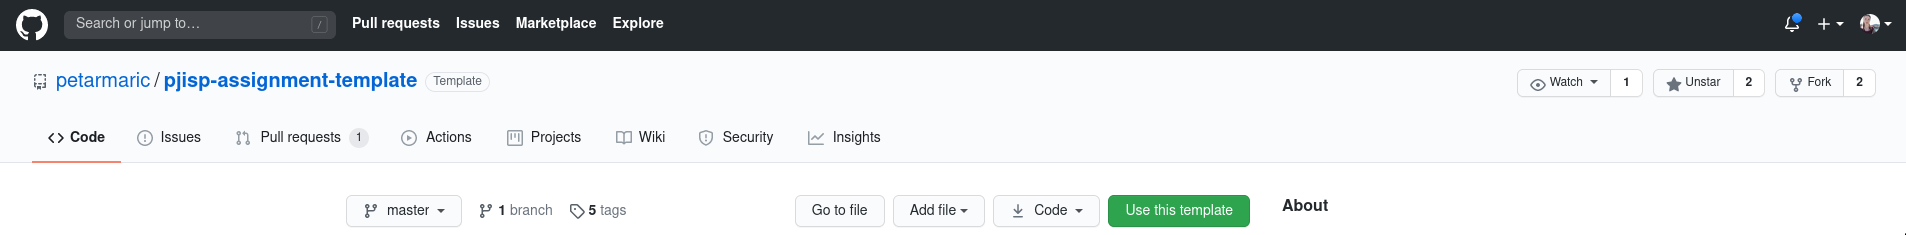
\includegraphics[width=\linewidth]{images/1.png}
    \caption{Kreiranje repozitorijuma - šablon}
\end{figure}

Nakon toga se korisniku prikazuje novi prozor, sa formom za kreiranje repozitorijuma iz šablona:

\begin{figure}[H]
    \centering
    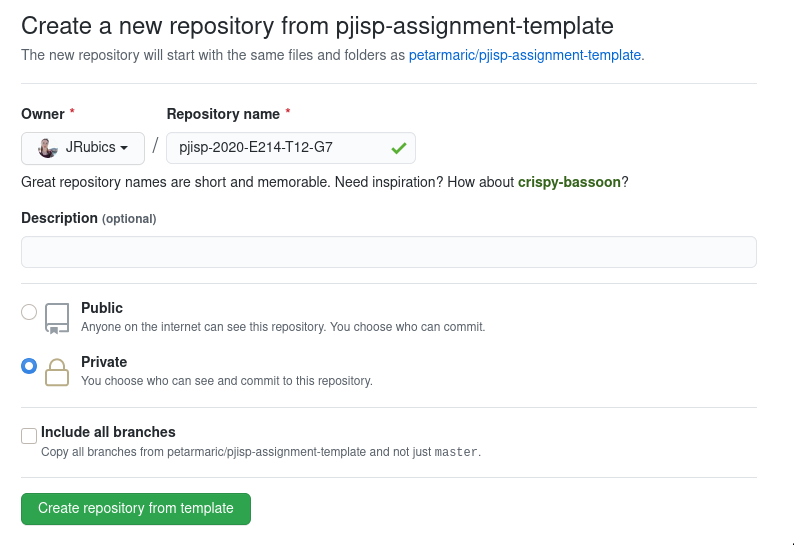
\includegraphics[width=0.7\linewidth]{images/2.png}
    \caption{Kreiranje repozitorijuma - popunjavanje forme}
\end{figure}

Od korisnika se očekuje da unese naziv repozitorijuma i da repozitorijum učini privatnim. Nakon pritiska na dugme \textit{``Create repository from template''} započinje generisanje repozitorijuma:

\begin{figure}[H]
    \centering
    
\includegraphics[width=0.6\linewidth]{images/3.png}
    \caption{Generisanje repozitorijuma}
\end{figure}

Po završetku kreiranja repozitorijuma, na korisnikovom nalogu se pojavljuje repozitorijum sa unetim nazivom i svim potrebnim datotekama za kreiranje zadatka za studente:

\begin{figure}[H]
    \centering
    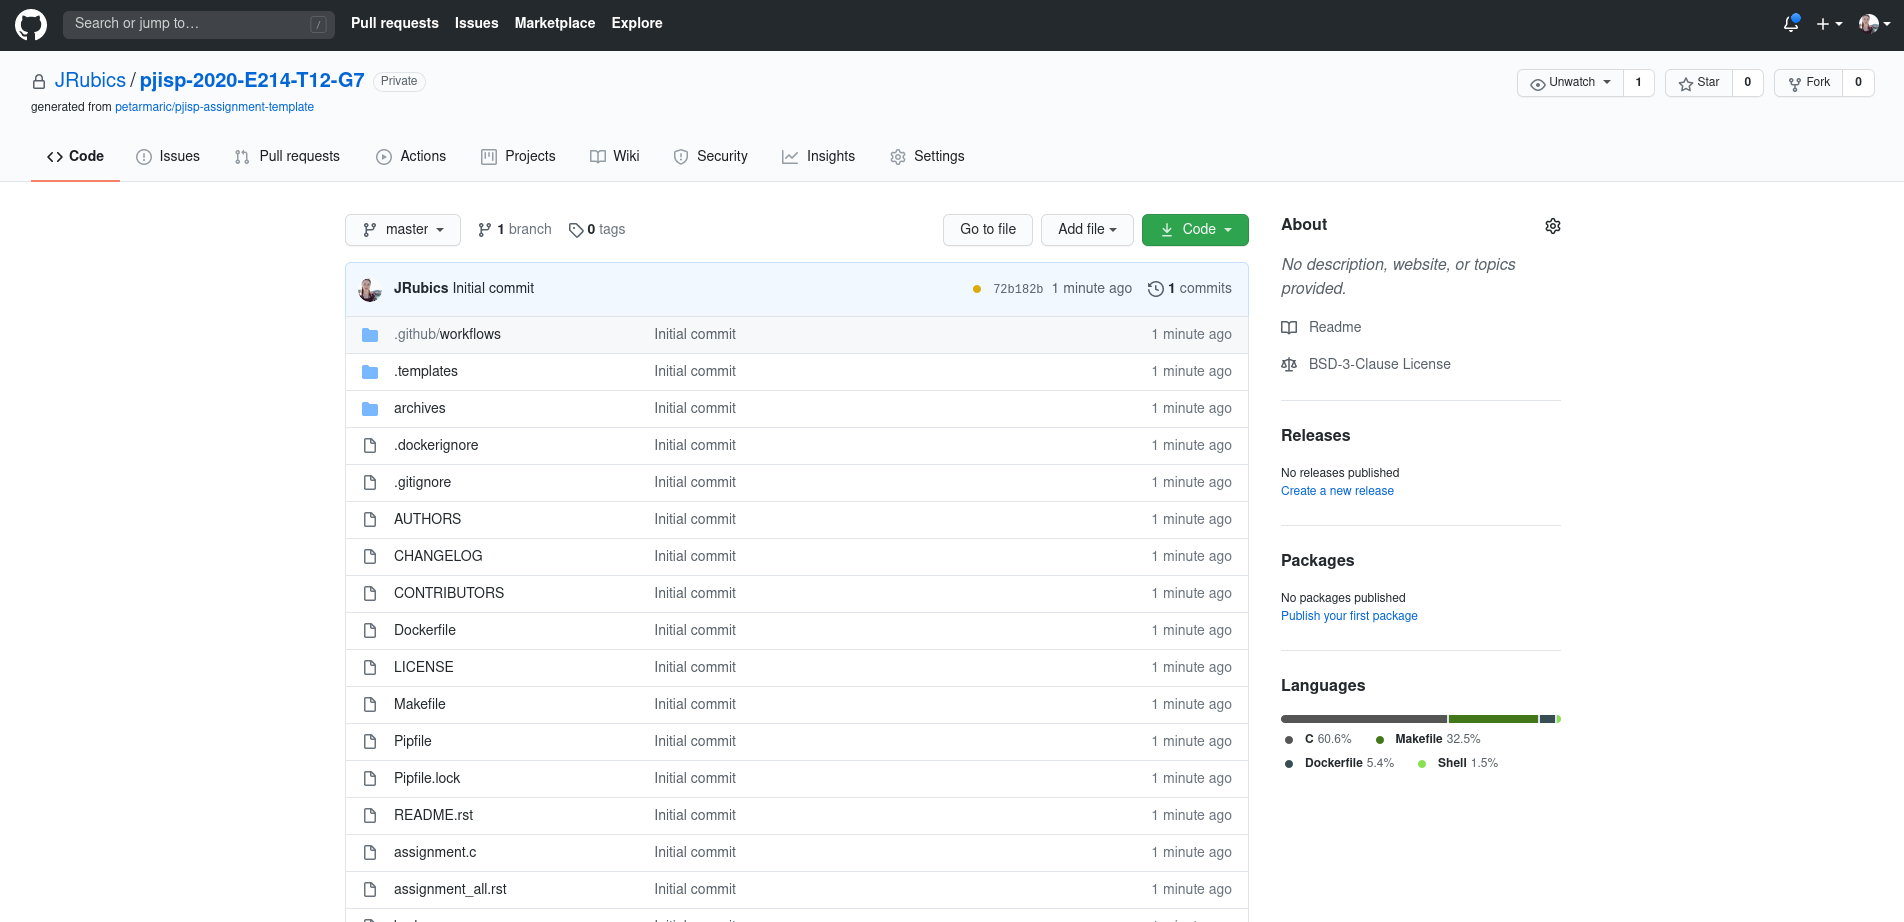
\includegraphics[width=\linewidth]{images/4.png}
    \caption{Repozitorijum}
\end{figure}

Između ostalog, generiše se i \textit{README.rst} datoteka na čijem početku se za sada ne nalazi ni jedan bedž:

\begin{figure}[H]
    \centering
    
\includegraphics[width=\linewidth]{images/5.png}
    \caption{\textit{README.rst} - nema bedž}
\end{figure}

Uporedno sa kreiranjem repozitorijuma, u odeljku \textit{Actions} se pokreću dva GitHub toka poslova:

\begin{enumerate}
    \item \textbf{Project create} - pri kreiranju repozitorijuma
    \item \textbf{PJISP Assignment} - pri inicijalnoj izmeni repozitorijuma (što je u ovom slučaju kreiranje)
\end{enumerate}

\begin{figure}[H]
    \centering
    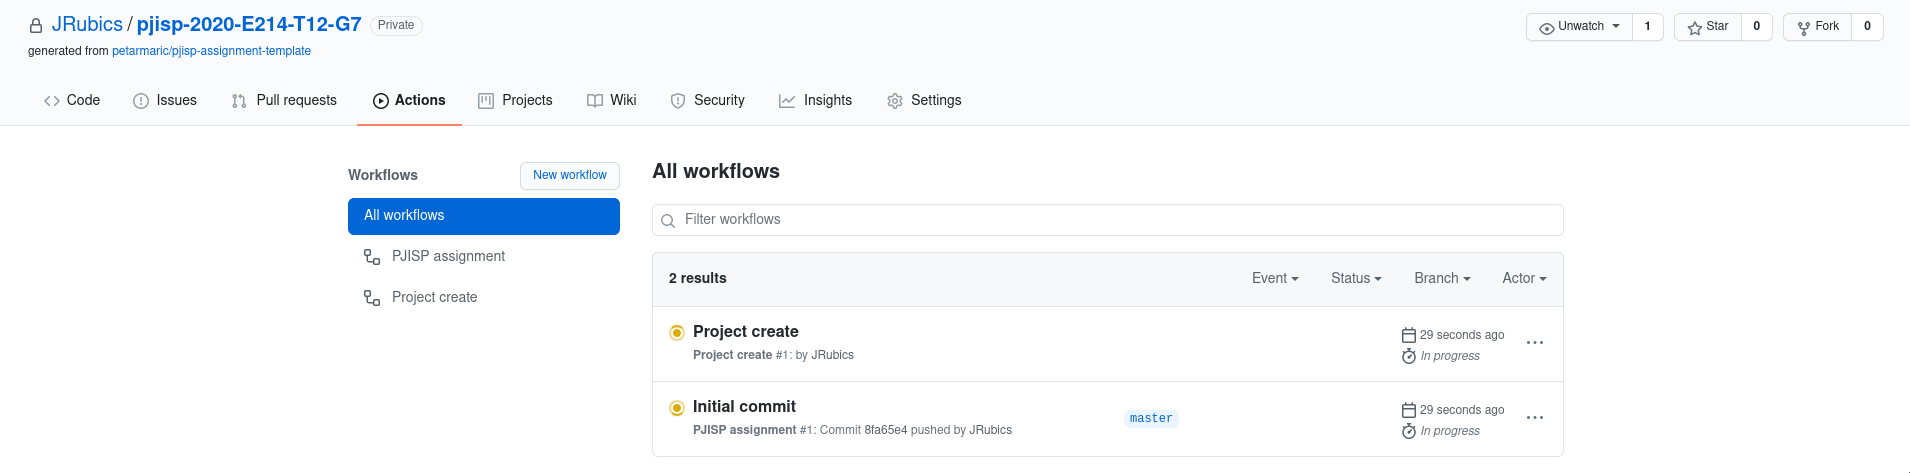
\includegraphics[width=\linewidth]{images/6.png}
    \caption{Prikaz tokova poslova}
\end{figure}

Svakom od tokova poslova moguće je pojedinačno pristupiti i pogledati njegov spisak poslova i koraka:

\begin{figure}[H]
    \centering
    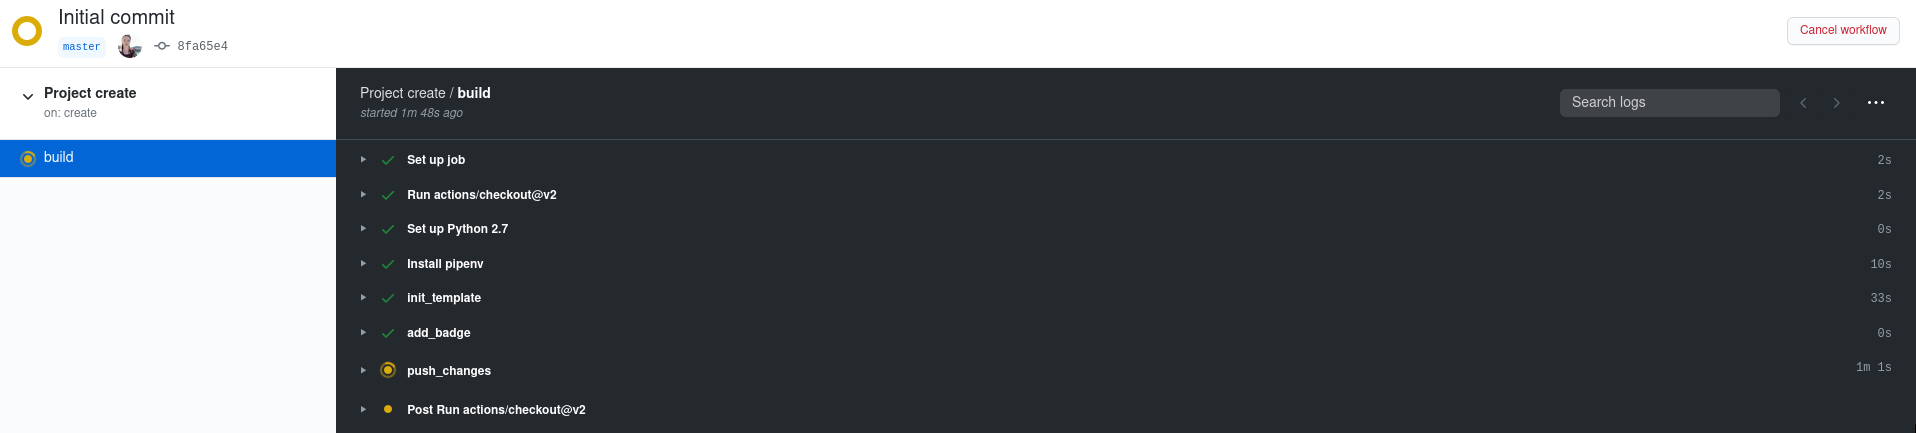
\includegraphics[width=\linewidth]{images/7.png}
    \caption{Prikaz poslova i koraka}
\end{figure}

Pritiskom mišem na neki od koraka, prikazuju se detalji njegovog izvršavanja:

\begin{figure}[H]
    \centering
    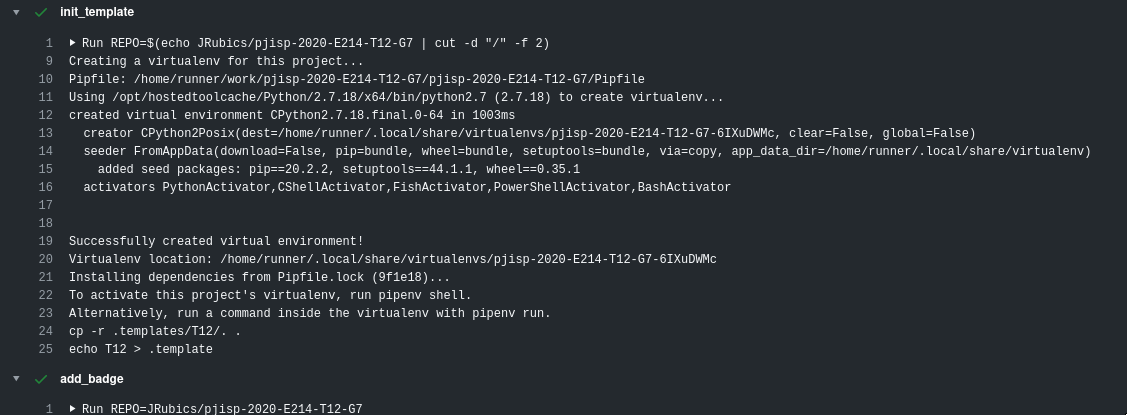
\includegraphics[width=\linewidth]{images/8.png}
    \caption{Detalji izvršavanja koraka}
\end{figure}

Nakon završetka izvršavanja, odeljak \textit{Actions} će imati jedan uspešno i jedan neuspešno završen tok poslova:

\begin{figure}[H]
    \centering
    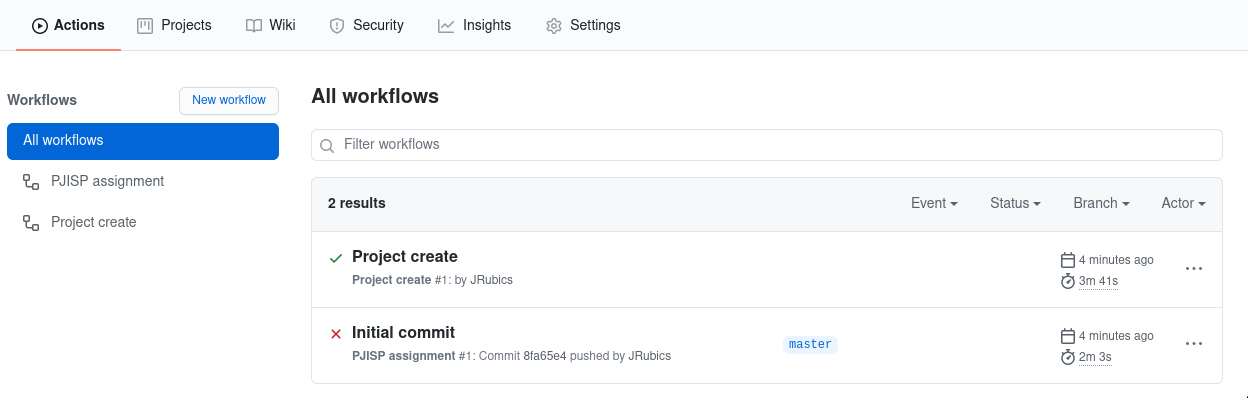
\includegraphics[width=\linewidth]{images/9.png}
    \caption{Završetak izvršavanja tokova poslova}
\end{figure}

Uspešno završen tok poslova je onaj koji se pokreće pri kreiranju repozitorijuma. Neuspešno završen tok posla je onaj koji testira ispravnost zadatka. Ovakav rezultat je i očekivan, pošto zaduženi iz nastavnog osoblja još uvek nije kreirao zadatak.

Odeljak \textit{PJISP Assignment} toka poslova prikazuje koji posao se neuspešno izvršio:

\begin{figure}[H]
    \centering
    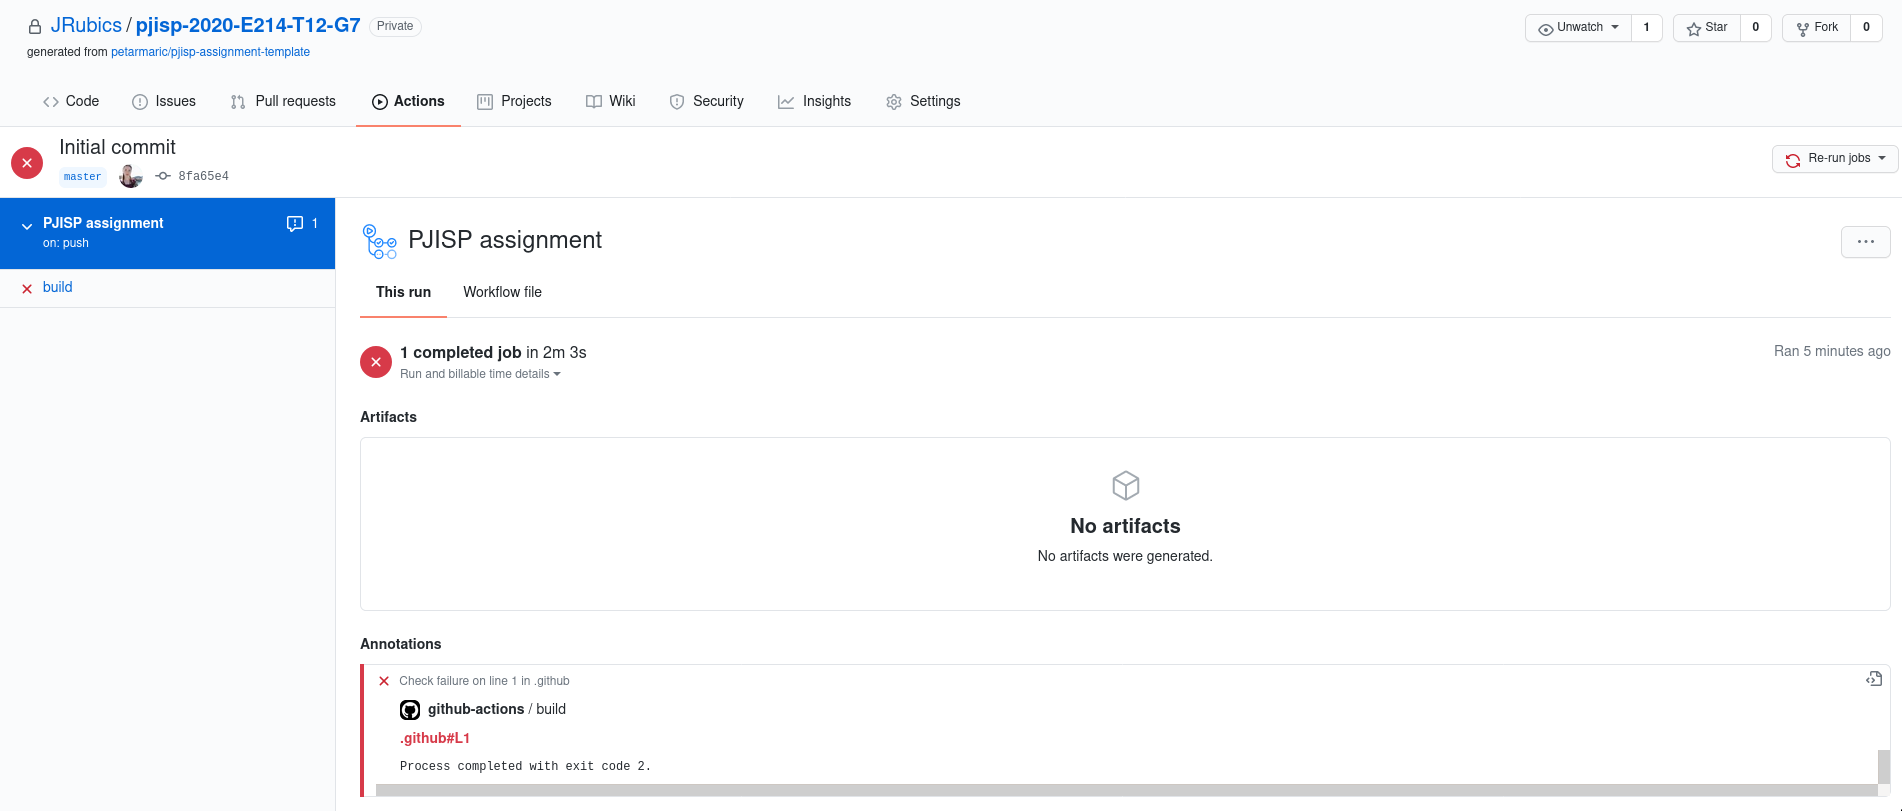
\includegraphics[width=\linewidth]{images/10.png}
    \caption{``PJISP assignment'' - neuspešno izvršavanje posla}
\end{figure}

Pritiskom mišem na neuspešno izvršen posao dobijaju se detalji o koraku koji je pouzrokovao neuspešno izvršavanje:

\begin{figure}[H]
    \centering
    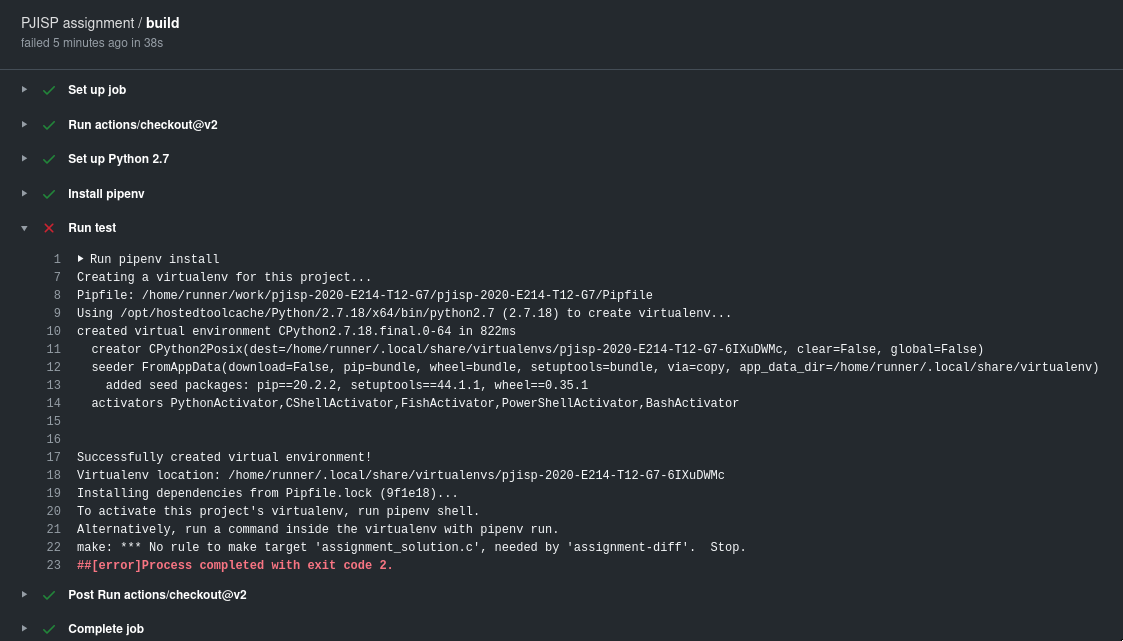
\includegraphics[width=\linewidth]{images/11.png}
    \caption{``PJISP assignment'' - detalji o neuspešnom izvršavanju posla}
\end{figure}

U ovom slučaju, to je nedostatak \textit{assignment\_solution.c} datoteke.

Pri izvršavanju \textit{Project create} toka posla, u \textit{README.rst} datoteku je dodat bedž na vrh. On za sada ima \textit{failing} vrednost zbog neuspešnog izvršavanja \textit{PJISP Assignment} toka poslova:

\begin{figure}[H]
    \centering
    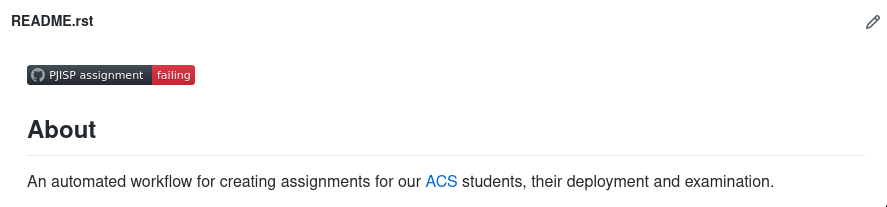
\includegraphics[width=\linewidth]{images/12.png}
    \caption{\textit{README.rst} - failing bedž}
\end{figure}

Dodate su i datoteke specifične za T12 test:

\begin{itemize}
    \item \textit{assignment\_solution.c}
    \item \textit{assignment.rst}
    \item \textit{assignment\_notes.rst}
    \item \textit{fixtures/stdio-numbers.yaml}
\end{itemize}

Ovim je završeno izvršavanje tokova poslova koji se pokreću pri kreiranju repozitorijuma, i on je spreman za pravljenje zadatka.

\section{Primer ispravnog kreiranja zadatka}

Kada autor zadatka izmeni sve potrebne datoteke i doda novu izmenu na GitHub, ponovo se pokreće \textit{PJISP Assignment} tok poslova:

\begin{figure}[H]
    \centering
    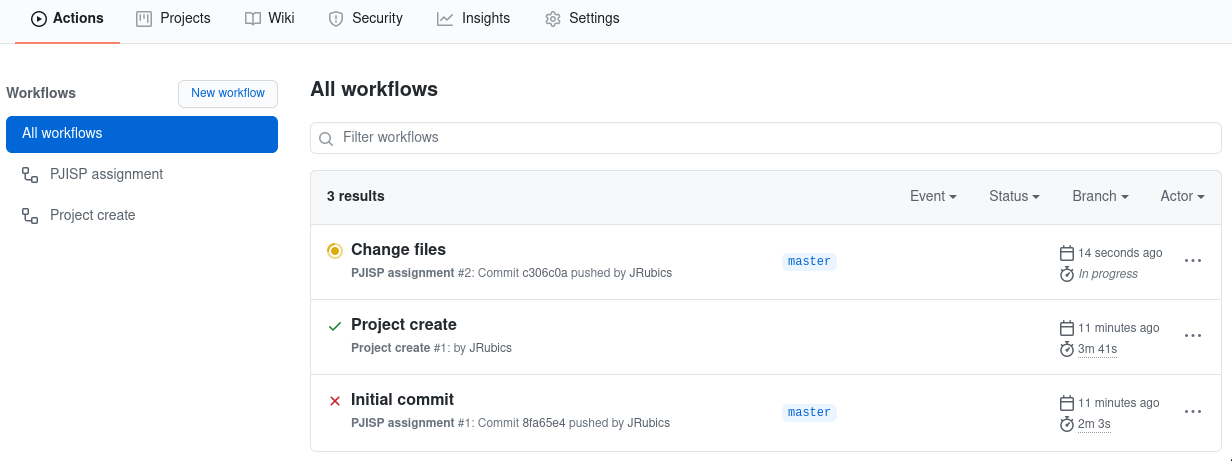
\includegraphics[width=\linewidth]{images/13.png}
    \caption{Prikaz tokova poslova}
\end{figure}

Pri uspešnom izvršavanju ovog toka poslova, bedž na početku \textit{README.rst} datoteke dobija \textit{passing} vrednost:

\begin{figure}[H]
    \centering
    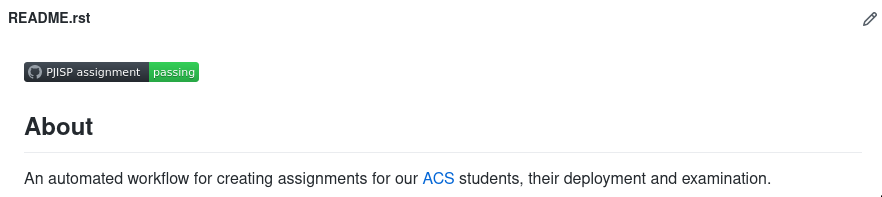
\includegraphics[width=\linewidth]{images/14.png}
    \caption{\textit{README.rst} - passing bedž}
\end{figure}

Ovim se uspešno završava kreiranje zadatka i on je spreman za pregledanje od strane nekog od nastavnika.

\section{Primeri grešaka}
Ova sekcija prikazuje po jedan primer za svaku od čestih grešaka koje nastavno osoblje može da napravi. Bilo koja slična greška, izazvaće isto ponašanje programa.

\subsection{Primer sa neispravnim testovima}

Ako se pri ponovnom pokretanju \textit{PJISP Assignment} toka poslova neki od testova ne izvrši uspešno, prikaz detalja o poslu će napisati razlog neuspešnog izvršavanja testa, a samim tim i toka posla:

\begin{figure}[H]
    \centering
    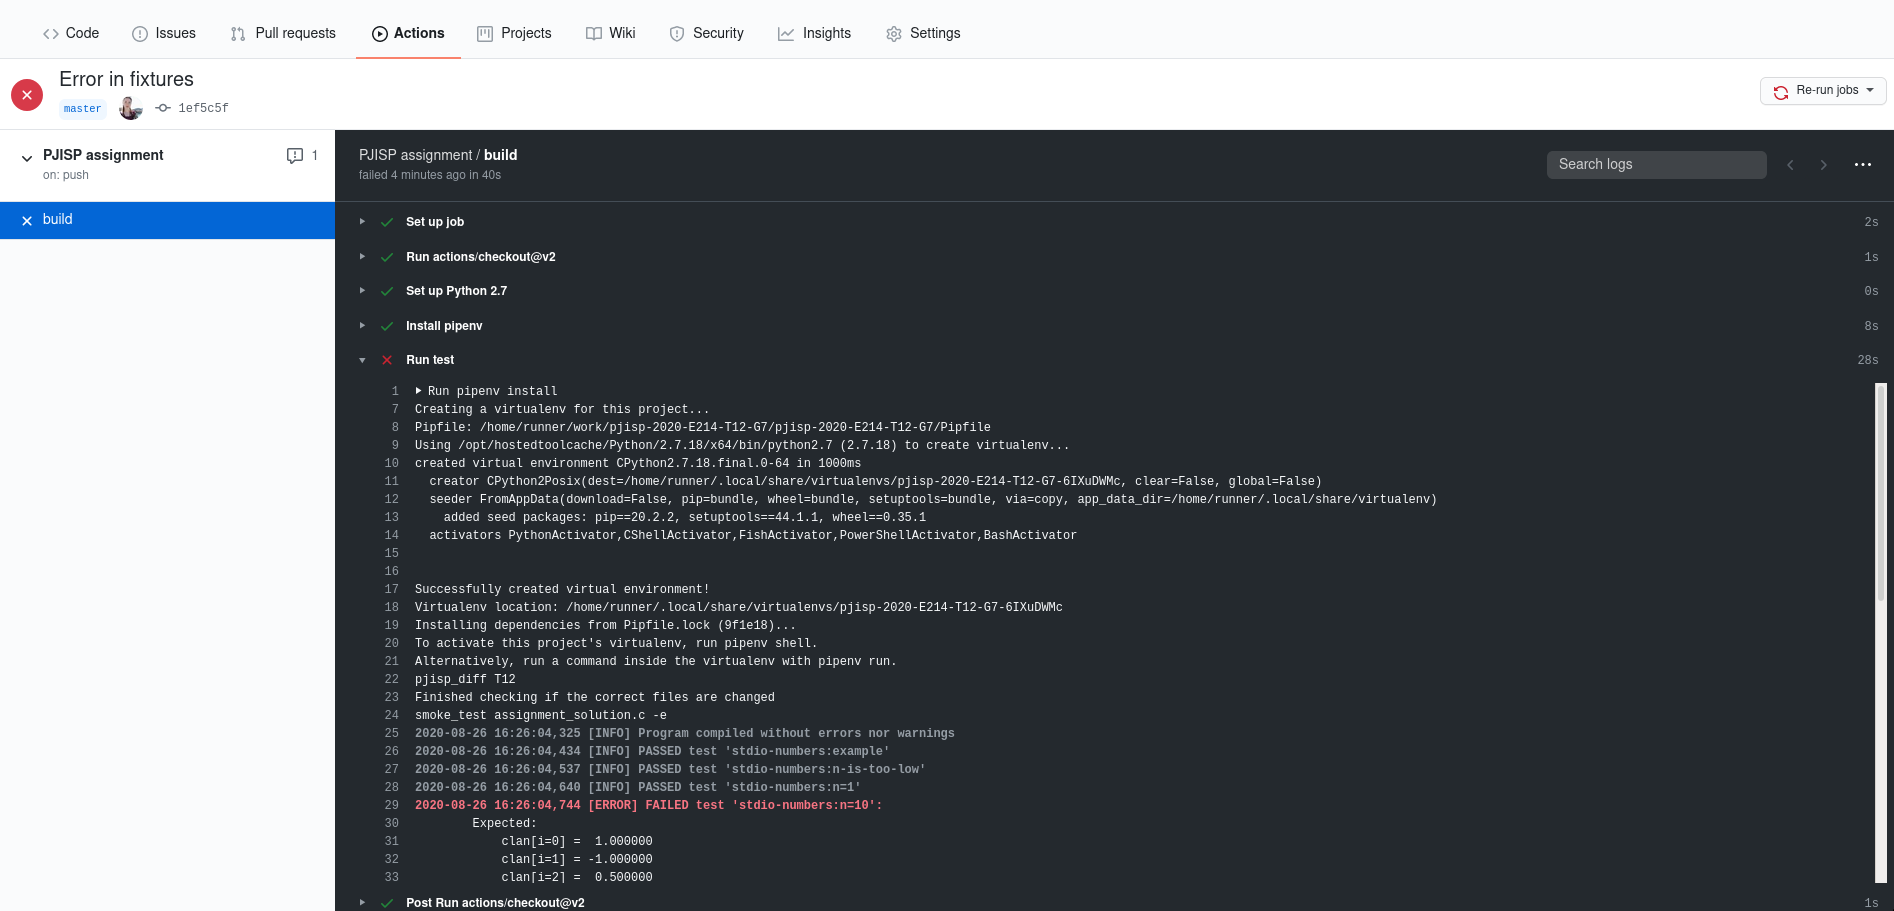
\includegraphics[width=\linewidth]{images/15.png}
    \caption{Kada se neki od testova neuspešno izvrši}
\end{figure}

U ovom primeru, test \texttt{stdio-numbers:n=10} imao je neočekivan izlaz i zato je dalje izvršavanje toka posla obustavljeno. Zbog toga, bedž na početku \textit{README.rst} datoteke dobija \textit{failing} vrednost.

\subsection{Primer sa neispravnim izmenama datoteka}

Ako se pri ponovnom pokretanju \textit{PJISP Assignment} toka poslova neka od datoteka koje je potrebno izmeniti ne izmeni ili se izmeni neka od datoteka koje se ne smeju menjati, prikaz detalja o poslu će obavestiti korisnika koja izmena nije odgovarajuća i obustaviće izvršavanje toka posla:

\begin{figure}[H]
    \centering
    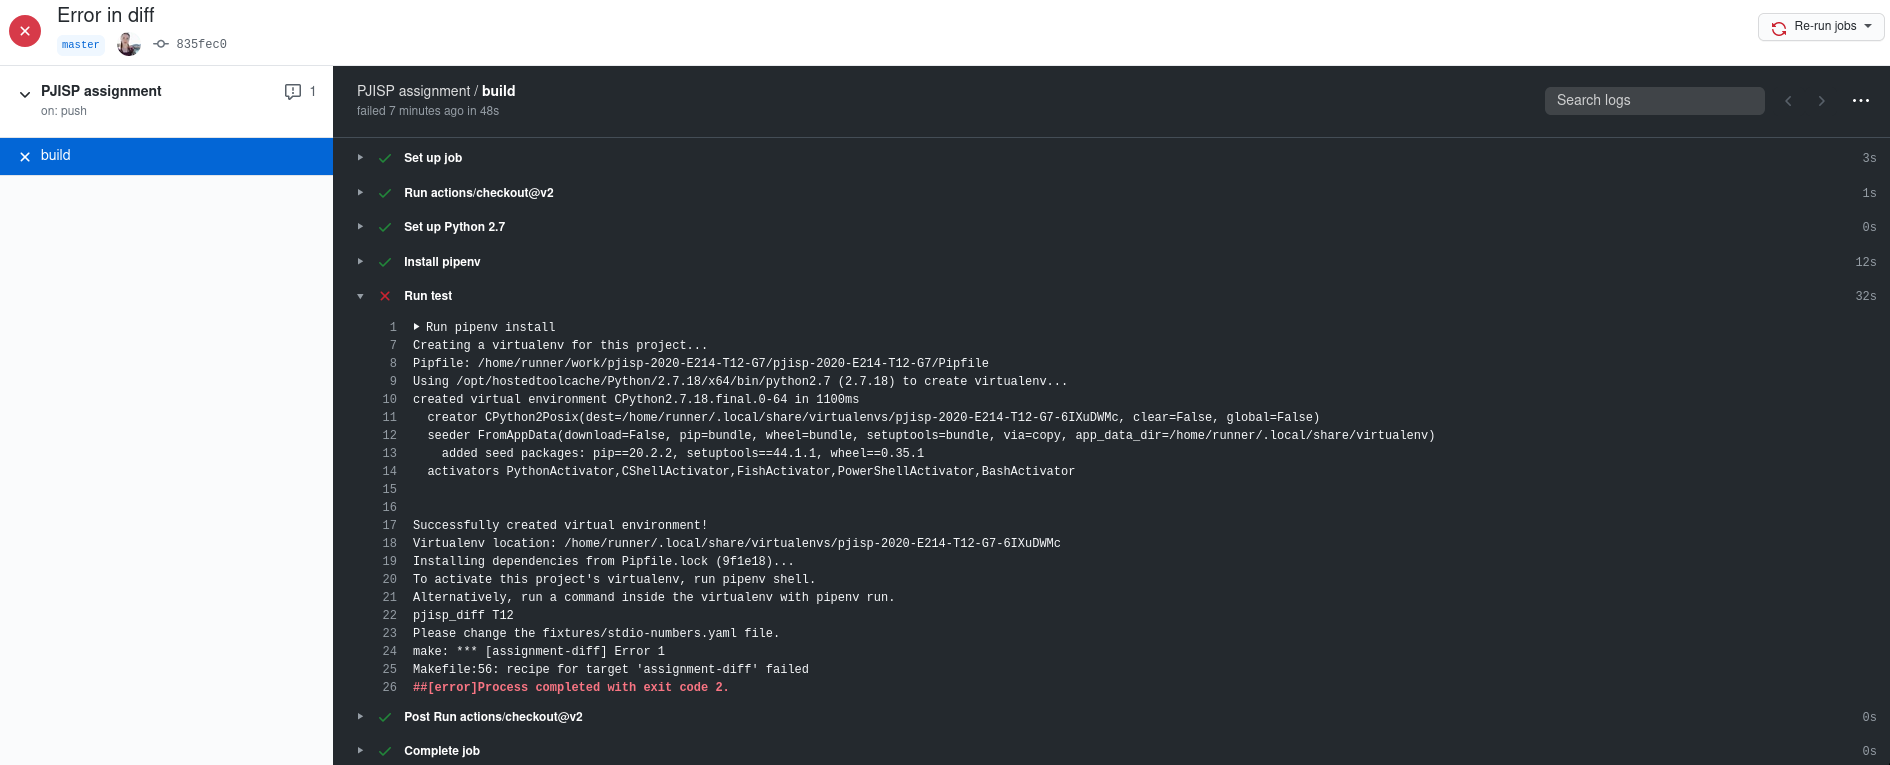
\includegraphics[width=\linewidth]{images/16.png}
    \caption{Kada se ne izmeni datoteka koju je potrebno izmeniti}
\end{figure}

U ovom primeru nije izmenjena datoteka \textit{fixtures/stdio-numbers.yaml} i zbog toga se prikazuje poruka \textit{``Please change the fixtures/stdio-numbers.yaml file.''} i vraća se izlazni kod \textit{1}, a zatim se tok poslova prekida sa izlaznim kodom \textit{2}. Zbog toga, bedž na početku \textit{README.rst} datoteke dobija \textit{failing} vrednost.

\subsection{Primer sa neispravnim nazivom repozitorijuma}

Pri kreiranju repozitorija, korisnik je u mogućnosti da unese neispravan naziv repozitorijuma i nakon toga pokrene kreiranje repozitorijuma:

\begin{figure}[H]
    \centering
    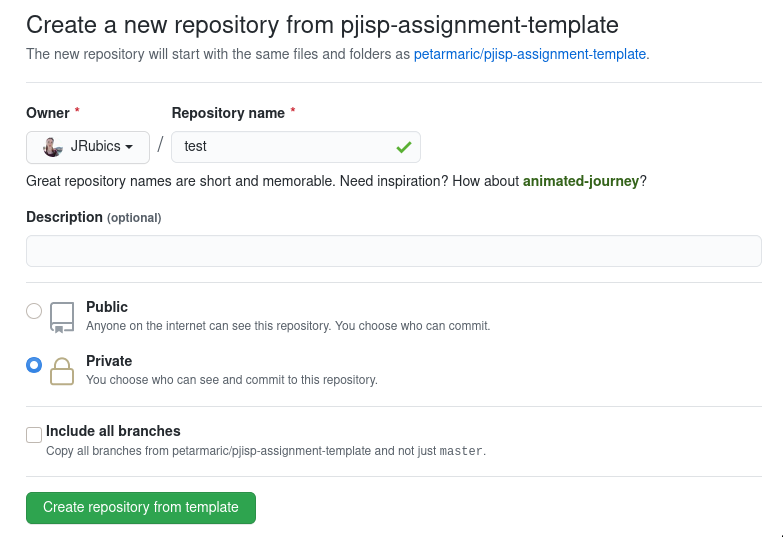
\includegraphics[width=0.7\linewidth]{images/17.png}
    \caption{Kreiranje repozitorijuma sa neispravnim nazivom}
\end{figure}

U tom slučaju će se \textit{Project create} tok podataka neuspešno izvršiti:

\begin{figure}[H]
    \centering
    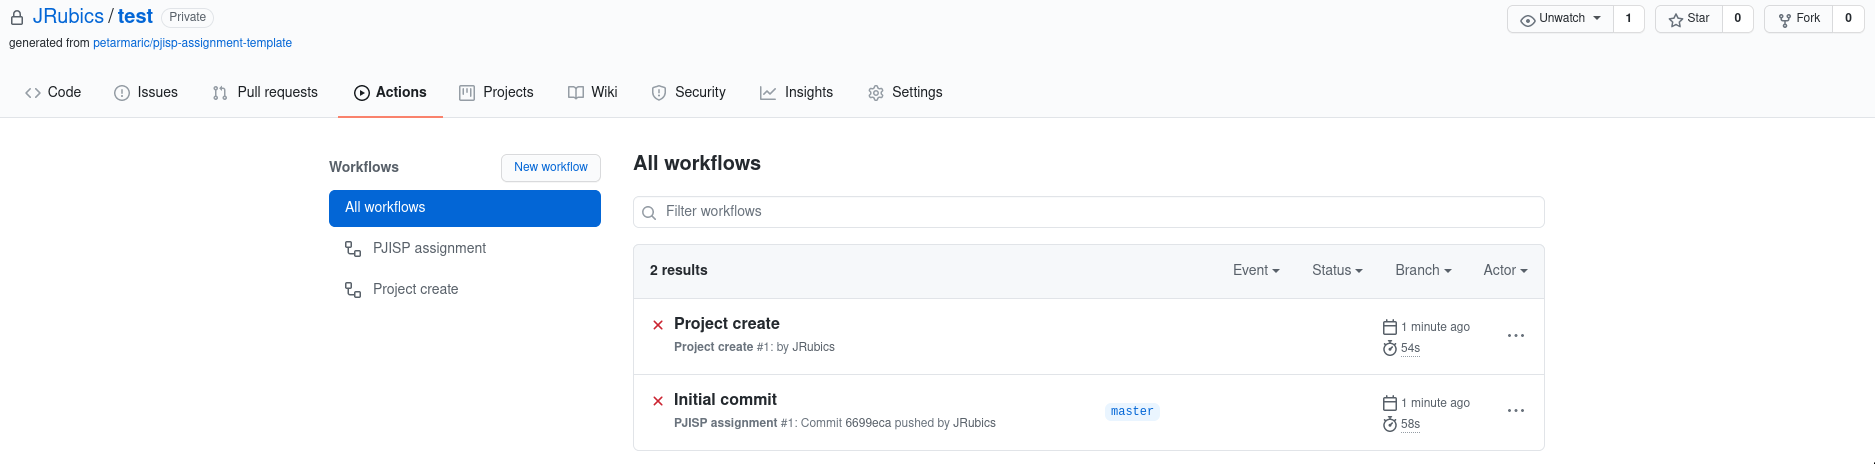
\includegraphics[width=\linewidth]{images/18.png}
    \caption{Prikaz tokova poslova}
\end{figure}

Prikaz detalja o koracima će dati korisniku razlog neuspešnog izvršavanja:

\begin{figure}[H]
    \centering
    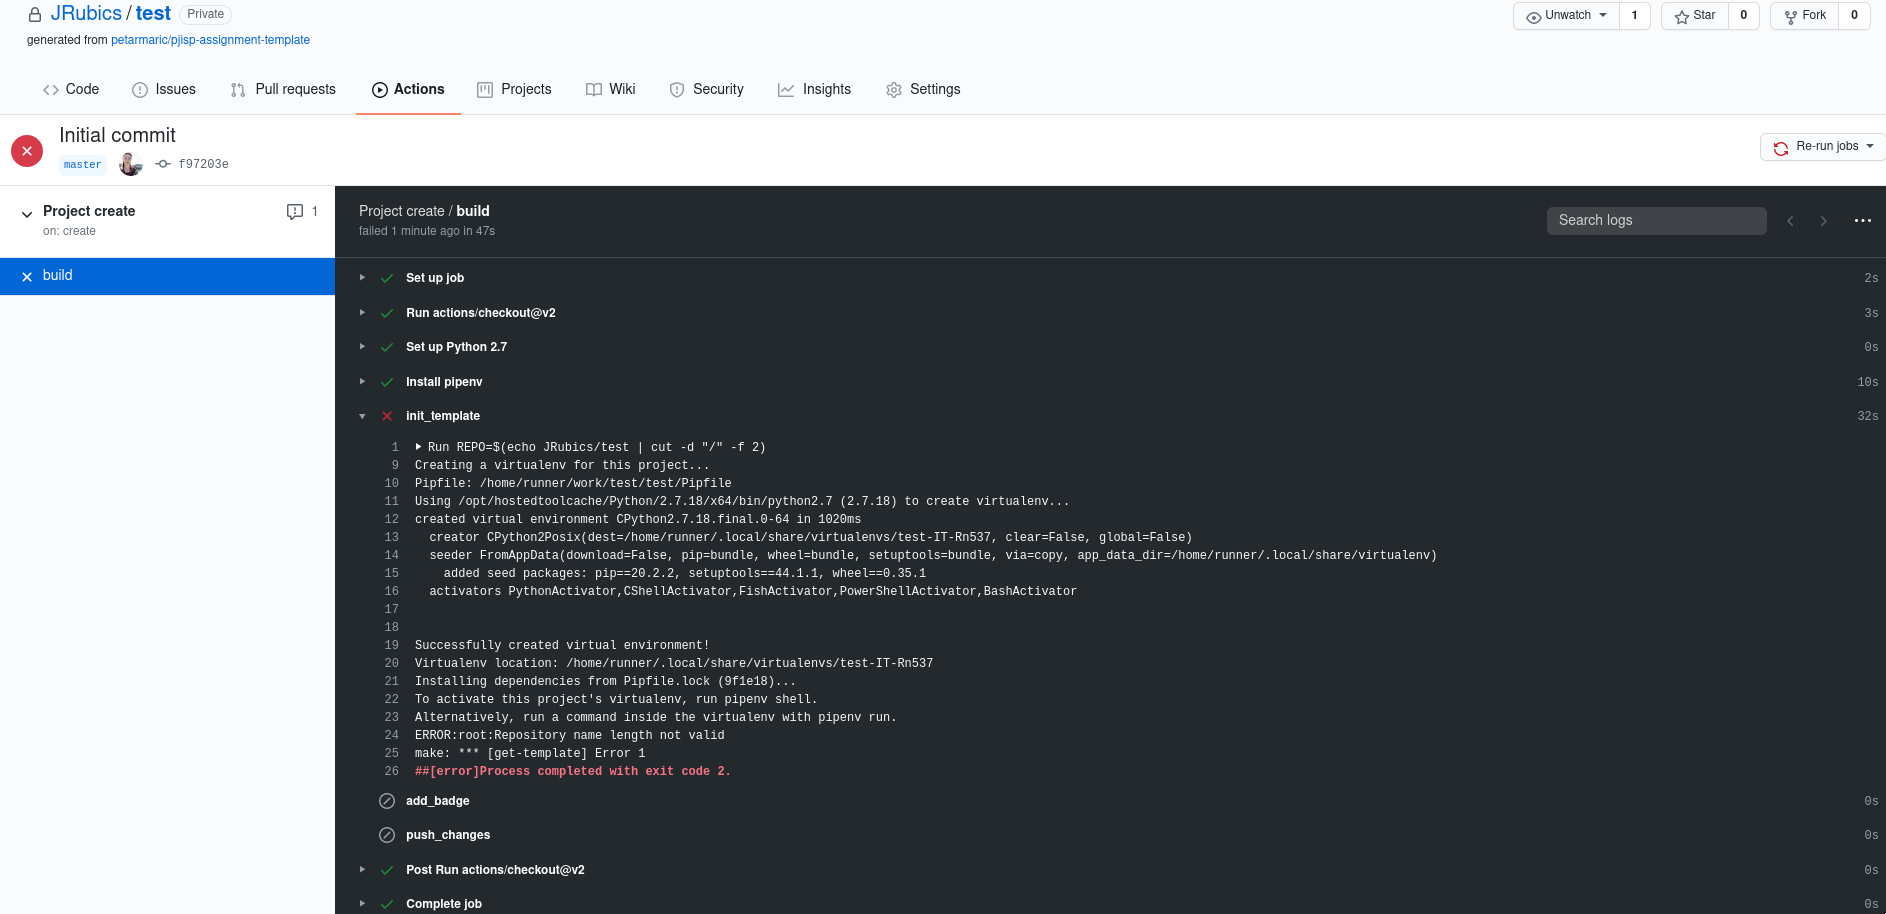
\includegraphics[width=\linewidth]{images/19.png}
    \caption{Kada dužina naziva repozitorijuma nije odgovarajuća}
\end{figure}

U ovom slučaju, to je neodgovarajuća dužina naziva repozitorijuma. Zbog toga, izvršavanje ovog toka posla se zaustavlja i preostala dva koraka posla u kojem je došlo do problema se neće izvršiti.

Ako je ipak dužina naziva dobra, ali neki od delova naziva ne odgovara šablonu davanja naziva repozitorijumu, ispisuje se poruka o tome i obustavlja se izvršavanje toka posla:

\begin{figure}[H]
    \centering
    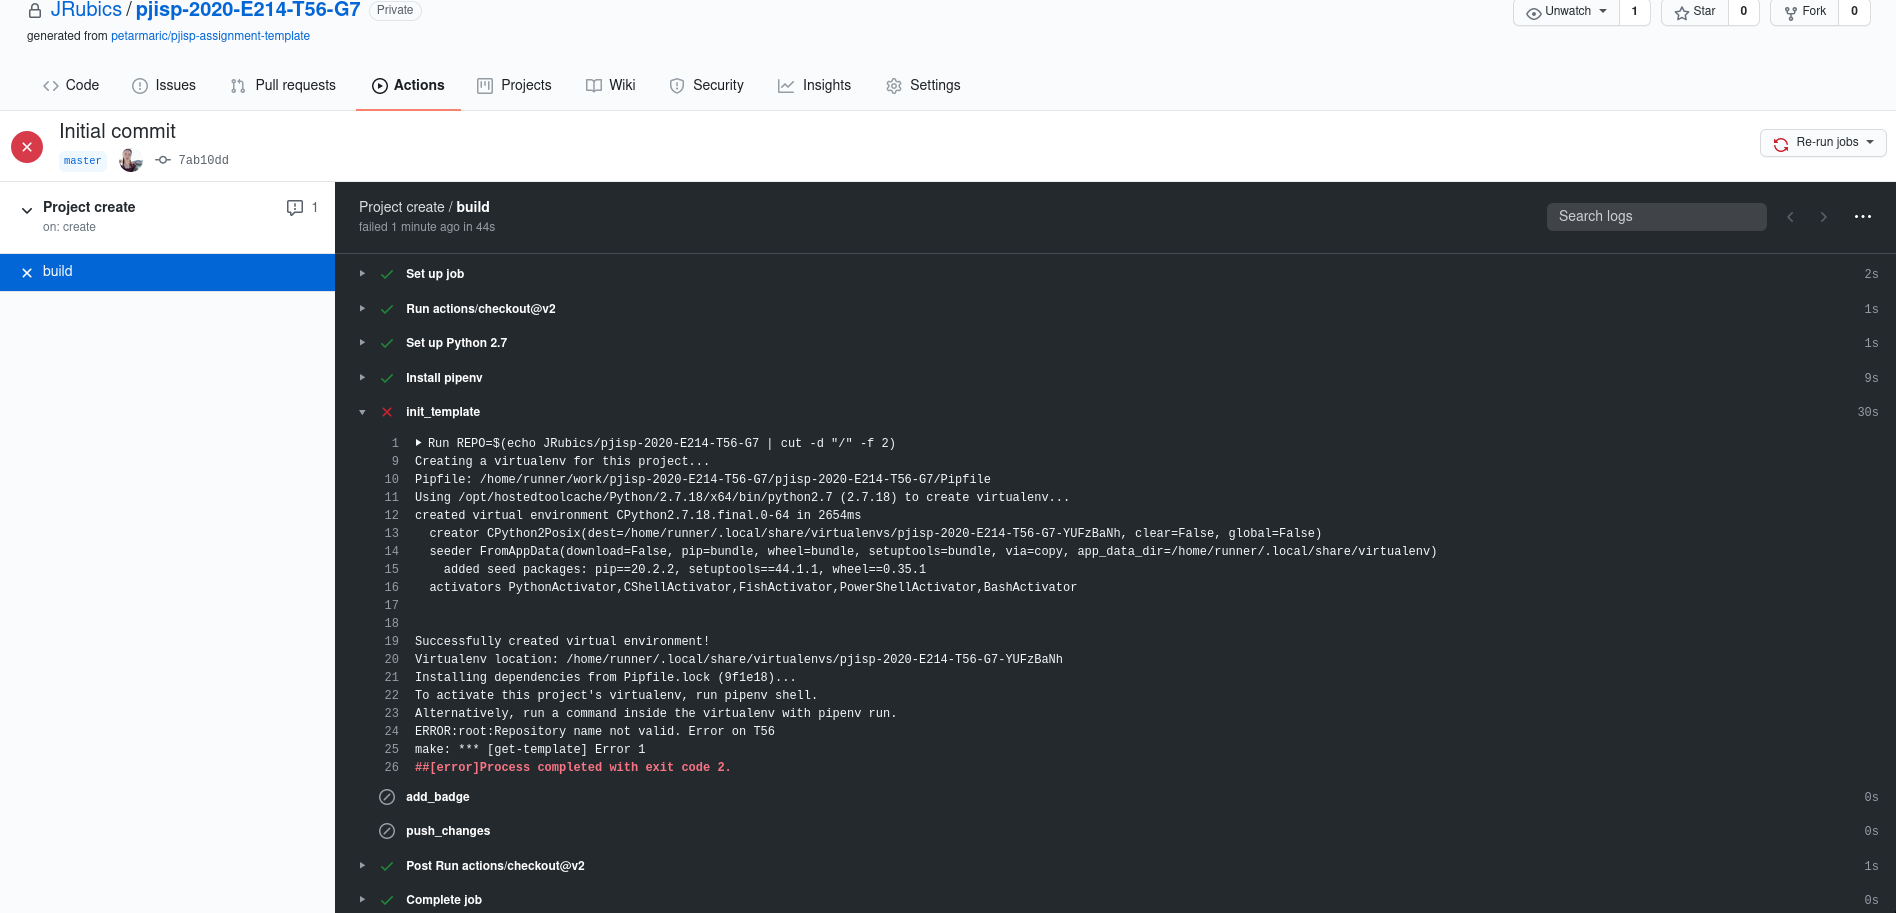
\includegraphics[width=\linewidth]{images/20.png}
    \caption{Kada naziv repozitorijuma nije odgovarajući}
\end{figure}

U ovom slučaju, problem je u tome što je kao naziv testa navedeno T56, iako su T12, T34 ili SOV jedine moguće opcije. Zbog toga korisnik dobija poruku \textit{``Repository name not valid. Error on T56''}.

\chapter{Diskusija i zaključci}

U ovom radu je predstavljen celokupan proces razvoja i unapređenja projekata otvorenog koda. Ideja je krenula od postojećeg projekta - \textit{pjisp-assignment-template} i u njega su se dodavale dodatne funkcionalnosti (\textit{pjisp-diff} i \textit{pjisp-template-name}). Svaka od tih funkcionalnosti je projekat za sebe, koji je odvojeno razvijan, a zatim integrisan sa malopre pomenutim projektom upotrebom GitHub tokova poslova i akcija. Jedan od postojećih Github akcija - \textit{poetry-publish} takođe igra važnu ulogu u razvoju projekata koji su nastali kao unapređenje \textit{pjisp-assignment-template} alata.

\section{Zaključci nakon upotrebe GitHub akcija}

Iz prethodnog pasusa vidimo da se mnoge nove funkcionalnosti u malopre pomenutom projektu oslanjaju na funkcionalnosti koje GitHub Actions servis nudi. Ovaj servis je dosta mlad, nastao je u novembru 2019. godine i to sa sobom donosi neke probleme. Još uvek nije u potpunosti pouzdan, pošto su neke od njegovih funkcionalnosti povremeno nedostupne \cite{status}. U trenutku pisanja ovog rada, funkcionalnosti su bile uglavnom dostupne:

\begin{figure}[H]
    \centering
    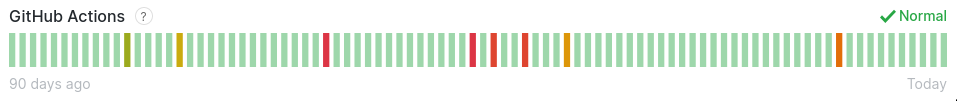
\includegraphics[width=\linewidth]{images/status.png}
    \caption{GitHub status, Avgust 2020}
\end{figure}

Svaki podeok na vremenskoj liniji (eng.\ \textit{timeline}) predstavlja jedan dan od proteklih 90 dana. Žute linije predstavljaju dane kada Akcije nisu bile dostupne manje od jednog sata. Narandžasta boja označava nedostupnost funkcionalnosti između jednog i dva sata, a crvena više od 2 sata.

Takođe, zbog brzog razvoja softvera, dokumentacija nije u svakom momentu usklađena sa alatom, pa to nekada može predstavljati problem za programere koji žele da koriste nove funkcionalnosti alata čim se one pojave.

I pored pomenutih problema, za potrebe ovakvog projekta, GitHub akcije donese mnoge beneficije i znatno olakšavaju razvoj i korišćenje svih prethodno pomenutih alata. Integracija alata je bila veoma jednostavna, pošto se šablon repozitorijum već nalazi na GitHub-u i onda nije bilo potrebno uvoditi dodatne alate u proces integracije.

Funkcionalnosti koje ove akcije uvode mogu znatno da smanje učestalost grešaka koje nastavno osoblje pravi prilikom kreiranja zadataka za studente. Olakšavaju i procenu spremnosti zadataka za davanje studentima, pošto bedž na početku \textit{README.rst} datoteke u repozitorijumu zadatka već naznačava da je zadatak prošao sve testove koje alat trenutno pokreće nad njim i da je spreman za pregledanje od strane drugog nastavnika.

\section{Dalji razvoj projekta}

Dalji razvoj ovog projekta bi pre svega obuhvatao praćenje razvoja GitHub akcija i implementaciju novih funkcionalnosti iz njih u projekat. Vremenom se mnoge funkcionalnosti menjaju i dodaju, i samim tim i korisničke akcije treba da se menjaju i poboljšavaju. Time će performanse i pouzdanost ovog projekta rasti.

Još neke stvari koje bi se mogle dodati bi bile dodatne provere prilikom kreiranja repozitorijuma ili dodavanja koda na repozitorijum. Ipak, svaki ovakav dodatak zahteva dodatno vreme izvršavanja toka posla. Zato, treba odrediti pravi odnos između benefita koji dodatne provere donose i vremena koje je potrebno za njihovo izvršavanje.

\chapter{Literatura}
\sloppy
\printbibliography[heading=none]

\end{document}
